\subsection{Strict morphisms of Fréchet spaces}

THEOREM 1. --- Let E and F be two Fréchet spaces and u a continuous linear mapping from E into F. The following conditions are equivalent :

\begin{enumerate}
\def\labelenumi{\alph{enumi})}
\item
  \(u\) is a strict morphism.
\item
  \(u\) is a strict morphism for the weakened topologies.
\item
  The image of u is closed in F.
\item
  \({}^t u\) is a strict morphism from \({\mathrm{F}}^{\prime }\) into \({\mathrm{E}}^{\prime }\) for the weak topologies.
\item
  The image of \({}^t u\) is closed in \({\mathrm{E}}^{\prime }\) for the weak topology \(\sigma \left( {{\mathrm{E}}^{\prime },\mathrm{E}}\right)\) .
\item
  The image of \({}^t u\) is closed in E' for the strong topology β(E', E).
\end{enumerate}

\(g)\) \({}^t u\) is a strict morphism from \(\mathrm{F}_c^\prime\) into \(\mathrm{E}_c^\prime\) (the duals endowed with the topology of compact convergence).

The equivalence of \(a\) , \(b\) ) and \(e\) ) follows from prop. 3 of IV, p.~28 and the remark preceding it. That of \(a\) ) and \(c\) ) is precisely cor. 3 of I, p.~19. The remark of IV, p.~28, also shows that \(d\) ) is equivalent to the fact that, the image of \(u\) is closed for the weakened topology \(\sigma(F, F')\) of \(F\) ; the equivalence of \(c\) ) and \(d\) ) then follows from prop. 2 of IV, p.~4.

We now prove the equivalence of \(e)\) and \(f)\) . It is enough to prove that \(f)\) implies \(e)\) . Suppose that the image of \({}^t u\) is closed for \(\beta(E', E)\) in \(E'\) . On account of the Banach-Dieudonné theorem (IV, p.~25, cor. 2), it is enough to prove that for every convex balanced neighbourhood \(U\) of \(0\) in \(E\) , the intersection \(B = {}^t u(F') \cap U\) is compact for \(\sigma(E', E)\) . The strong dual \(E_b'\) of the Fréchet space \(E\) is complete (IV, p.~22, prop. 2), hence the closed subset \(B\) of \(E_b'\) is complete, and so the normed space \(E_B'\) is complete (III, p.~8, corollary). Let \((V_n)\) be a decreasing sequence forming a fundamental system of neighbourhoods of \(0\) in \(F\) . Then \(F'\) is the union of sets \(C = V_n^\circ\) which are compact for \(\sigma(F', F)\) , hence \(E_B' = \bigcup B_n\) , with \(B_n = E_B' \cap {}^t u(C_n)\) . Since \(E_B'\) is a Baire space, and each of the sets \(B_{n}\) is convex balanced and closed, there exists a real number r \textgreater{} 0 and an integer n such that \(B \subset r \cdot B_{n}\) . Then we have \(\mathbf{B} = \mathbf{U}^{\circ} \cap {}^{t} u(r \cdot C_{n})\) ; since the sets \(U^{\circ}\) and \(r \cdot C_{n}\) are compact and \({}^{t} u\) is continuous for the weak topologies, B is compact for \(\sigma(\mathrm{E}', \mathrm{E})\) . This completes the proof of the equivalence of e) and f).

Finally the equivalence of \(g\) ) and the preceding conditions follows from prop. 18 of GT, X, § 2, No.~10 and the following lemma.

Lemma 1. --- Let E and F be two Hausdorff locally convex and quasi-complete spaces and u a continuous linear mapping from E into F. For \({}^t u\) to be a strict morphism from \(F_{c}'\) into \(E_{c}'\) , it is necessary and sufficient that the image \(u(E)\) of u be closed, and that every compact subset of \(u(E)\) be the image under u of a compact subset of E.

By Mackey's th. (IV, p.~2, th. 1) and the fact that on \(\mathrm{E}'\) (resp. F) the topology of compact convergence coincides with that of convex compact convergence (IV, p.~4), we can identify E (resp. F) with the dual \(\mathrm{E}_c'\) (resp. \(\mathrm{F}_c'\) ). Then \(u\) is the transpose of \({}^t u\) , and the equicontinuous subsets of E (resp. F) are the relatively compact sets. Lemma 1 then follows from prop. 2 (IV, p.~27), since \(u(\mathrm{E})\) is closed in F if and only if it is closed for the weakened topology \(\sigma(\mathrm{F}, \mathrm{F}')\) (IV, p.~4, prop. 2).

COROLLARY 1. --- Under the hypothesis of th. 1, the following conditions are equivalent :

\begin{enumerate}
\def\labelenumi{(\roman{enumi})}
\item
  \(u\) is a strict injective morphism;
\item
  \({}^{t}u\) is a strict surjective morphism for the weak topologies.
\item
\({}^{t}u\) is surjective.
\end{enumerate}

The implication (i) \(\Rightarrow\) (ii) follows immediately from the equivalence of conditions \(a\) , \(d\) ) and \(e\) ) of th. 1 and from IV, p.~6, prop. 5. It is clear that (ii) implies (iii). Finally, we prove that (iii) implies (i): if \({}^t u\) is surjective \(u\) is a strict morphism by the equivalence of \(a\) ) and \(e\) ) in th. 1; that \(u\) is injective follows from prop. 5 of IV, p.~6.

COROLLARY 2. --- Under the hypothesis of th. 1, the following conditions are equivalent :

\begin{enumerate}
\def\labelenumi{(\roman{enumi})}
\item
  \(u\) is surjective;
\item
  \(u\) is a strict surjective morphism;
\item
  \({}^t u\) is a strict injective morphism for the weak topologies.
\end{enumerate}

The equivalence of (i) and (ii) follows from Banach's th. (I, p.~17, th. 1).

In view of the equivalence of \(a\) and \(c\) in th. 1, condition (ii) says that \(u\) is a strict morphism and that its image is dense in F for \(\sigma(F, F')\) . The equivalence of (ii) and (iii) then follows from the equivalence of \(a\) and \(d\) in th. 1 and from prop. 5 of IV, p.~6.

If \(u: \mathrm{E} \to \mathrm{F}\) is a strict morphism of Fréchet spaces, the transpose \({}^t u\) is not necessarily a strict morphism from \(\mathrm{F}_b'\) into \(\mathrm{E}_b'\) (IV, p.~62, exerc. 3). However, we have the following partial result :

COROLLARY 3. --- Under the hypotheses of th. 1, the following property implies the properties a) to g):

\begin{enumerate}
\def\labelenumi{\alph{enumi})}
\setcounter{enumi}{7}
\tightlist
\item
  \({}^{t}u\) is a strict morphism from \(F_{b}^{\prime}\) into \(E_{b}^{\prime}\) .
\end{enumerate}

When E and F are both Banach spaces, or both Montel spaces, property \(h)\) is equivalent to the properties \(a)\) to \(g)\) of th. 1.

Suppose that \({}^t u\) is a strict morphism from \(\mathrm{F}_b'\) into \(\mathrm{E}_b'\) . We shall prove that the image H of \({}^t u\) is closed in \(\mathrm{E}_b'\) , from which the first assertion of cor. 3 will follow.

Let G be the closure of the image of u in F; the space G, with the topology induced by that of F assigned to it, is a Fréchet space. The mapping \(u: E \to F\) factorizes as \(u = j \circ v\) where j is the canonical injection from G into F and where \(v \in \mathcal{L}(E; G)\) . Then we have \({}^t u = {}^t v \circ {}^t j\) , where \({}^t j\) is surjective, by Hahn-Banach th. (II, p.~24, prop. 2); also, \({}^t v\) is injective since \(v(E)\) is dense in G (IV, p.~6, prop. 5). By hypothesis, the mapping \({}^t u\) from \(F_{b}'\) onto H is open; since \({}^t j\) is surjective and continuous, the mapping \({}^t v\) induces a homeomorphism from \(G_{b}'\) onto H. But the dual \(G_{b}'\) of the Fréchet space G is complete (IV, p.~22, prop. 2); consequently H is complete, hence closed in \(E_{b}'\) .

If E and F are Montel spaces, the strong topology on \(E'\) (resp. \(F'\) ) coincides with the topology of compact convergence, and h) is just a reformulation of g).

If E and F are Banach spaces, so are \(E_{b}^{\prime}\) and \(F_{b}^{\prime}\) , and condition h) is equivalent to f) by the equivalence of a) and c) applied to \(u: F_{b}^{\prime} \to E_{b}^{\prime}\) .

COROLLARY 4. --- Suppose E and F are Banach spaces. For \({}^t u\) to be surjective, it is necessary and sufficient that there exist a real number \(r > 0\) such that \(\| x\| \leqslant r.\| u(x)\|\) for all \(x\in E\) .

This is simply a reformulation of the equivalence of the conditions (i) and (iii) of cor. 1.

COROLLARY 5. --- Let E and F be two Fréchet spaces and u a continuous linear mapping

from E into F. The following conditions are equivalent :

\begin{enumerate}
\def\labelenumi{\alph{enumi})}
\item
  \(u\) is an isomorphism from E onto F.
\item
  u is an isomorphism from E onto F for the weakened topologies.
\item
  \({}^t u\) is an isomorphism from \({\mathrm{F}}^{\prime }\) onto \({\mathrm{E}}^{\prime }\) for the weak topologies.
\item
  \({}^{t}u\) is an isomorphism from \(F'\) onto \(E'\) for the strong topologies.
\item
  \({}^t u\) is an isomorphism from \({\mathrm{F}}_{c}^{\prime }\) onto \({\mathrm{E}}_{c}^{\prime }\) .
\end{enumerate}

Since an isomorphism is none other than a strict bijective morphism, the equivalence of \(a)\) and \(b)\) follows from the equivalence of conditions \(a)\) and \(b)\) of th. 1.

It is clear that a) implies each of the conditions c), d) and e).

Conversely, suppose that one of the conditions \(c\) ), \(d\) or \(e\) ) is satisfied. It follows from th. 1 and its cor. 3 that \(u\) is a strict morphism from E into F, and \({}^t u\) is evidently bijective. Let N (resp. I) be the kernel (resp. the image) of \(u\) . Since \({}^t u\) is bijective, we have \(\operatorname{Im} {}^t u = \operatorname{E}'\) and \(\operatorname{Ker} {}^t u = \{0\}\) , and so \(\mathrm{N}^\circ = \mathrm{E}'\) and \(\mathrm{I}^\circ = \{0\}\) by prop. 2 of IV, p.~27. But N (resp. I) is a closed vector subspace of E (resp. F), and the theorem of bipolars (II, p.~44) implies that \(\mathrm{N} = \{0\}\) and \(\mathrm{I} = \mathrm{F}\) , hence \(u\) is bijective. We have therefore proved that \(u\) is an isomorphism.

\subsection{Criteria for surjectivity}

PROPOSITION 4. --- Let E and F be two Fréchet spaces, and u a continuous linear mapping from E into F. The following conditions are equivalent :

\begin{enumerate}
\def\labelenumi{(\roman{enumi})}
\item
  u is surjective.
\item
  For every semi-norm \(p \in \mathbf{S}(\mathbf{E})\) , there exists \(q \in \mathbf{S}(\mathbf{F})\) such that we have \(|f| \leqslant q\) for every linear form \(f \in \mathbf{F}'\) satisfying \(|f \circ u| \leqslant p\) .
\item
  For every semi-norm \(p \in \mathrm{S}(\mathrm{E})\) , there exists \(q \in \mathrm{S}(\mathrm{F})\) satisfying the following property: if a linear form \(f \in F'\) satisfies \(|f \circ u| \leqslant p\) , then f is null on points where q is null and for all \(y \in F\) , \(r \in \mathrm{S}(\mathrm{F})\) , there exists \(x \in E\) with \(r(u(x) - y) = 0\) .
\item
  For every semi-norm \(p \in \mathrm{S}(\mathrm{E})\) , we have
\end{enumerate}

\[
\sup_{\substack{f\in \mathbf{F}^{\prime}\\ |f\circ u|\leqslant p}}\big|f(y)\big| <   + \infty \quad \text{for all} \quad y\in \mathbf{F}  .\tag{1}
\]

We shall prove the proposition according to the following logical scheme

\pandocbounded{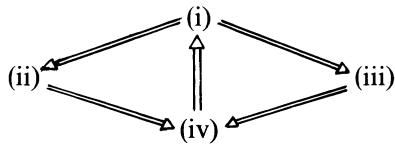
\includegraphics[keepaspectratio]{images/part002_fd83f186.jpg}}

If \(u\) is surjective, it is a strict morphism (IV, p.~28, th. 1) then for every semi-norm \(p \in \mathrm{S}(\mathrm{E})\) , there exists a semi-norm \(q \in \mathrm{S}(\mathrm{F})\) such that, for all \(y \in \mathrm{F}\) satisfying \(q(y) \leqslant 1\) , there exists \(x \in \mathrm{E}\) satisfying \(p(x) \leqslant 1\) and \(u(x) = y\) . We deduce immediately that (i) implies (ii) and (iii). It is clear that (ii) implies (iv).

To prove that (iii) implies (iv), let \(p\) and \(q\) be as in (iii). Let \(y \in \mathbf{F}\) , by (iii), there exists \(x\) in \(\mathbf{E}\) such that \(q(u(x) - y) = 0\) . If \(f \in \mathbf{F}'\) satisfies \(|f \circ u| \leqslant p\) , then we have \(f(u(x) - y) = 0\) , hence

\[
\left| f (y) \right| = \left| f (u (x)) \right| \leqslant p (x)
\]

and the relation (1) is satisfied.

Finally we prove that (iv) implies (i). Let \(p \in \mathrm{S}(\mathrm{E})\) and let \(q\) be the superior envelope of the functions \(|f|\) for \(f \in \mathrm{F}'\) satisfying \(|f \circ u| \leqslant p\) . By (iv), \(q\) is finite on \(\mathrm{F}\) , and is evidently a lower semi-continuous semi-norm on \(\mathrm{F}\) ; since \(\mathrm{F}\) is barrelled (III, p.~25, corollary), we have \(q \in \mathrm{S}(\mathrm{F})\) . Let \(\mathbf{B}_p\) (resp. \(\mathbf{B}_q\) ) denote the set of all \(x \in \mathrm{E}\) (resp. \(y \in \mathrm{F}\) ) such that \(p(x) \leqslant 1\) (resp. \(q(y) \leqslant 1\) ). We have \(q \circ u \leqslant p\) , and so \(u(\mathbf{B}_p) \subset \mathbf{B}_q\) . The polar of \(u(\mathbf{B}_p)\) in \(\mathrm{F}'\) consists of linear forms \(f \in \mathrm{F}'\) such that \(|f \circ u| \leqslant p\) , hence \(|f| \leqslant q\) ; in other words, we get \(u(\mathbf{B}_p)^{\circ} \subset \mathbf{B}_q^{\circ}\) , and finally that \(\overline{u(\mathbf{B}_p)} = \mathbf{B}_q\) follows from the theorem of bipolars (II, p.~45, cor. 3). If \(\mathrm{U}\) is a neighbourhood of 0 in \(\mathrm{E}\) , there exists \(p \in \mathrm{S}(\mathrm{E})\) such that \(\mathbf{B}_p \subset \mathbf{U}\) , hence \(\overline{u(\mathbf{U})}\) contains the neighbourhood \(\mathbf{B}_q\) of 0 in \(\mathrm{F}\) . This implies that \(u\) is surjective (I, p.~17, th. 1).

COROLLARY. --- Suppose E and F are Banach spaces. The following conditions are equivalent :

\begin{enumerate}
\def\labelenumi{(\roman{enumi})}
\item
  \(u\) is surjective.
\item
  There exists a real number \(r > 0\) , such that \(\| f \| \leqslant r\) . \(\| {}^t u(f) \|\) for all \(f \in \mathbf{F}'\) .
\item
  For all \(y \in F\) , we have \(\sup_{\substack{f\in \mathbf{F}^{\prime}\\ |f\circ u|\leqslant 1}} |f(y)| < +\infty\) .
\end{enumerate}

The conditions (ii) and (iii) are in fact reformulations of conditions (ii) and (iv) of prop. 4 for Banach spaces.

\section{COMPACTNESS CRITERIA}

\subsection{General remarks}

Let A be a subset of a topological space E. For a sequence \((x_{n})_{n\in\mathbf{N}}\) of points of A to have a point x of E as a limit point, it is necessary and sufficient that the following condition is satisfied (GT, I, § 7, No.~3):

\begin{enumerate}
\def\labelenumi{(\Alph{enumi})}
\tightlist
\item
  For every integer \(m \geqslant 0\) and every neighbourhood \(\mathbf{U}\) of \(x\) , there exists an integer \(n \geqslant m\) such that \(x_{n} \in \mathbf{U}\) .
\end{enumerate}

A sequence of the form \((y_{k})_{k\in\mathbb{N}}\) with \(y_{k}=x_{n_{k}}\) for a strictly increasing sequence \((n_{k})_{k\in\mathbb{N}}\) of positive integers is called an extracted sequence of the sequence \((x_{n})_{n\in\mathbb{N}}\) . If there exists an extracted sequence of the sequence \((x_{n})_{n\in\mathbb{N}}\) which converges to x, then x is a limit point of \((x_{n})\) ; conversely, if x has a countable fundamental system of neighbourhoods, and x is the limit point of the sequence \((x_{n})\) , then there exists an extracted sequence of \((x_{n})\) converging to x.

On account of GT, IX, § 2, No.~9, corollary, we conclude that when E is metrizable, the following conditions are equivalent :

\begin{enumerate}
\def\labelenumi{\alph{enumi})}
\item
  the set A is relatively compact in E;
\item
  every infinite sequence of points of A has a limit point in E;
\item
  from every infinite sequence of points of A, we can extract a sequence which converges to a point of E.
\end{enumerate}

In this section, we shall extend this criterion to certain non metrizable topological vector spaces. The following proposition enables us to reduce the study of compact sets to that of weakly compact sets in a number of cases.

PROPOSITION 1. --- Let E be a Hausdorff locally convex space, and A a subset of E. Let \(E_{\sigma}\) denote the space E with the weakened topology.

\begin{enumerate}
\def\labelenumi{\alph{enumi})}
\item
  If every infinite sequence of points of \(\mathbf{A}\) has a limit point in \(\mathbf{E}\) , then \(\mathbf{A}\) is precompact in \(\mathbf{E}\) .
\item
  In order that A be relatively compact in E, it is necessary and sufficient that it is precompact in E and relatively compact in \(E_{\sigma}\) .
\end{enumerate}

We shall prove \(a)\) by reductio ad absurdum. If \(A\) is not precompact, then by th. 3 of GT, II, § 3, No.~7, it follows that there exists a symmetric convex neighbourhood \(V\) of 0 in \(E\) such that \(A\) cannot be covered by a finite number of translates of \(V\) .

In other words, if \(x_{0}, x_{1}, \ldots, x_{n-1}\) are points of A, then \(A \not\subset \bigcup_{0 \leqslant i < n} (x_{i} + V)\) and so there exists a point \(x_{n}\) of A such that \(x_{n} - x_{i} \notin V\) for \(0 \leqslant i < n\) . Then, by induction on the integer n, we can construct an infinite sequence \((x_{n})_{n \in \mathbb{N}}\) of points of A such that \(x_{n} - x_{m} \notin V\) whenever n \textgreater{} m; since V is symmetric, we also have \(x_{m} - x_{n} \notin V\) for \(m \neq n\) and the sets \(x_{n} + \frac{1}{2}V\) are disjoint. For every point x in E, there exists at most one integer \(n \geqslant 0\) such that \(x_{n} \in x + \frac{1}{2}V\) , hence the sequence \((x_{n})_{n \in \mathbb{N}}\) does not have any limit point. This proves a).

Now suppose that A is precompact in E and is contained in a compact subset B of \(E_{\sigma}\) . Then B is complete in \(E_{\sigma}\) , hence also in E (IV, p.~5, Remark 2). We have \(\overline{A} \subset B\) , hence A is relatively compact in E. The converse is evident and b) follows.

\subsection{Simple compactness of sets of continuous functions}

In this section, X denotes a compact space and \(\mathcal{C}_{s}(X)\) the space of continuous functions on X, with values in the field K (equal to R or C). The space \(\mathcal{C}_{s}(X)\) is assigned the topology of simple convergence on X.

PROPOSITION 2. --- Let D be a dense subset of X and A a subset of the space \(\mathcal{C}_{s}(X)\) . The following conditions are equivalent :

\begin{enumerate}
\def\labelenumi{(\roman{enumi})}
\item
  A is relatively compact in \(\mathcal{C}_s(\mathbf{X})\) .
\item
  From every infinite sequence of elements of \(\mathbf{A}\) , we can extract a sequence converging in \(\mathcal{C}_s(\mathbf{X})\) .
\item
  Every infinite sequence of elements of \(\mathbf{A}\) has a limit point in \(\mathcal{C}_s(\mathbf{X})\) .
\item
  Let \((f_n)_{n\in \mathbb{N}}\) be a sequence of functions belonging to A and \((x_m)_{m\in \mathbb{N}}\) a sequence of points of D. If the iterated limits
\end{enumerate}

\[
\gamma = \lim _ {m \rightarrow \infty} \lim _ {n \rightarrow \infty} f _ {n} (x _ {m}), \quad \delta = \lim _ {n \rightarrow \infty} \lim _ {m \rightarrow \infty} f _ {n} (x _ {m})
\]

exist, then they are equal. In addition, we have \(\sup_{f\in \mathbf{A}}|f(x)| < +\infty\) for all \(x\in \mathbf{X}\) .

\begin{enumerate}
\def\labelenumi{(\roman{enumi})}
\tightlist
\item
  \(\Rightarrow\) (ii): let \(\overline{\mathbf{A}}\) be the closure of \(\mathbf{A}\) in \(\mathcal{C}_s(\mathbf{X})\) . Assume that \(\mathbf{A}\) is compact, and consider a sequence of functions \(f_n \in \mathbf{A}\) (for \(n \in \mathbf{N}\) ). Let \(\phi\) be the continuous mapping \(x \mapsto (f_n(x))_{n \in \mathbf{N}}\) from \(\mathbf{X}\) into the metrizable space \(\mathbf{K}^{\mathbf{N}}\) . The image \(\mathbf{X}'\) of \(\mathbf{X}\) under \(\phi\) is a compact metrizable space, since \(\mathbf{X}\) is compact. Let \(\mathbf{E}\) be the closed subspace of \(\mathcal{C}_s(\mathbf{X})\) consisting of continuous functions \(f\) on \(\mathbf{X}\) such that the relation \(\phi(x) = \phi(y)\) implies \(f(x) = f(y)\) for every pair of points \(x, y\) in \(\mathbf{X}\) . By cor. 2 of GT, I, § 9, No.~4 and prop. 3 of GT, I, § 5, No.~2, the mapping \(f' \mapsto f' \circ \phi\) is a homeomorphism \(\phi^*\) from \(\mathcal{C}_s(\mathbf{X}')\) onto E. Hence the set \(\mathbf{A}' = (\phi^*)^{-1}(\overline{\mathbf{A}})\) is compact in \(\mathcal{C}_s(\mathbf{X}')\) , and it is clear that there exist elements \(f_n'\) in \(\mathbf{A}'\) such that \(\phi^*(f_n') = f_n' \circ \phi\) is equal to \(f_n\) .
\end{enumerate}

Since \(X'\) is a compact metrizable space, there exists a countable dense subset \(D'\) in \(X'\) (GT, IX, §2, No.~8, prop. 12 and §2, No.~9, prop. 16). Let \(T_{1}\) (resp. \(T_{2}\) ) be the topology on \(A'\) induced by the topology of simple convergence on \(D'\) (resp. \(X'\) ). Then \(T_{1}\) is metrizable, \(T_{2}\) is compact and finer than \(T_{1}\) , hence \(T_{1}\) and \(T_{2}\) coincide; in other words, \(A'\) is a compact metrizable subspace of \(\mathcal{C}_{s}(X')\) . Therefore, there exists a sequence \((f_{n_k}^{\prime})\) extracted from \((f_n^{\prime})\) and converging to an element \(f^{\prime}\) of \(\mathcal{C}_s(\mathbf{X}')\) . Therefore, the sequence \((f_{n_k})\) converges to \(f = f' \circ \phi\) in \(\mathcal{C}_s(\mathbf{X})\) .

\begin{enumerate}
\def\labelenumi{(\roman{enumi})}
\setcounter{enumi}{1}
\item
  \(\Rightarrow\) (iii): this is clear.
\item
  \(\Rightarrow\) (iv): suppose that every infinite sequence of elements of A has a limit point in \(\mathcal{C}_s(\mathbf{X})\) . Let \(x \in \mathbf{X}\) . The mapping \(\phi_x: f \mapsto f(x)\) from A into K is continuous. Consequently, every infinite sequence in \(\phi_x(\mathbf{A})\) has a limit point; since the field K (equal to R or C) is metrizable, the set \(\phi_x(\mathbf{A})\) is relatively compact in K, hence bounded. In other words, we have \(\sup_{f \in \mathbf{A}} |f(x)| < \infty\) .
\end{enumerate}

Let \(f_n, x_m, \gamma\) and \(\delta\) be as in (iv). Let \(f\) be a limit point of the sequence \((f_n)\) in \(\mathcal{C}_s(\mathbf{X})\) , and let \(x\) be a limit point of the sequence \((x_m)\) in the compact space \(\mathbf{X}\) . For every \(m\) , the mapping \(h \mapsto h(x_m)\) from \(\mathcal{C}_s(\mathbf{X})\) into \(\mathbf{K}\) is continuous. In view of the hypotheses, we have \(f(x_m) = \lim_{n \to \infty} f_n(x_m)\) , and hence \(\gamma = \lim_{m \to \infty} f(x_m)\) ; since \(f: \mathbf{X} \to \mathbf{K}\) is continuous and \(x\) is a limit point of the sequence \((x_m)\) , we get \(\gamma = f(x)\) . In an analogous way, we prove the equality \(\delta = f(x)\) , whence \(\gamma = \delta\) .

\begin{enumerate}
\def\labelenumi{(\roman{enumi})}
\setcounter{enumi}{3}
\tightlist
\item
  \(\Rightarrow\) (i): suppose that the set of numbers \(f(x)\) , as \(f\) ranges over \(\mathbf{A}\) , is bounded in \(\mathbf{K}\) for all \(x\in \mathbf{X}\) . This is equivalent to assuming that the closure \(\overline{\mathbf{A}}\) of \(\mathbf{A}\) in the product space \(\mathbf{K}^{\mathbf{X}}\) is compact (GT, I, § 9, No.~5). Suppose that \(\mathbf{A}\) is not relatively compact in \(\mathcal{C}_s(\mathbf{X})\) . This means that there exists a function \(u\in \overline{\mathbf{A}}\) and a point \(a\in \mathbf{X}\) such that \(u\) is not continuous at \(a\) . Hence there exists a real number \(\varepsilon >0\) such that in every neighbourhood \(\mathrm{U}\) of \(a\) , there exists a point \(x\) with \(|u(x) - u(a)|\geqslant \varepsilon\) .
\end{enumerate}

We shall construct by induction a sequence \((x_{n})_{n\in \mathbf{N}}\) of points in \(\mathbf{D}\) and a sequence \((f_n)_{n\in \mathbf{N}}\) of elements of \(\mathbf{A}\) , satisfying the following relations:

\[
\left| u (x _ {m}) - u (a) \right| \geqslant \varepsilon \quad \text { for } \quad m \geqslant 1;\tag{$(1)_{m}$}
\]

\[
\left| u (x _ {i}) - f _ {m} (x _ {i}) \right| \leqslant \frac {1}{m + 1} \text { for } 0 \leqslant i \leqslant m - 1;\tag{$(2)_{m}$}
\]

\[
\left| f _ {m} (x _ {i}) - f _ {m} (a) \right| \leqslant \frac {1}{i + 1} \quad \text { for } \quad 0 \leqslant m \leqslant i.\tag{$(3)_{m,i}$}
\]

We take \(x_0 = a\) with \(f_0\) arbitrary in A (the set A is not empty, otherwise it will be relatively compact in \(\mathcal{C}_s(\mathbf{X})\) ). Let \(n \geqslant 1\) and \(x_0, x_1, \ldots, x_{n-1}, f_0, f_1, \ldots, f_{n-1}\) satisfy relations \((1)_m, (2)_m\) for \(1 \leqslant m < n\) and \((3)_{m,i}\) for \(0 \leqslant m \leqslant i < n\) . Since \(u\) belongs to \(\overline{\mathbf{A}}\) , there exists \(f_n \in \mathbf{A}\) satisfying \((2)_n\) . Let \(V_n\) be the set of all \(x \in X\) such that \(|f_m(x) - f_m(a)| \leqslant \frac{1}{n+1}\) for \(0 \leqslant m \leqslant n\) . Since \(f_n\) is continuous, \(V_n\) is a neighbourhood of \(a\) ; choose a point \(x_n\) in \(D \cap V_n\) such that \(|u(x_n) - u(a)| \geqslant \varepsilon\) , hence \((1)_n\) and \((3)_{m,n}\) are satisfied. Therefore, the construction can be continued.

Since \(u(\mathbf{X})\) is a compact subset of \(\mathbf{K}\) , there exists a sequence \((y_k)\) extracted from \((x_m)\) and such that the limit \(\gamma = \lim_{k\to \infty}u(y_k)\) exists. By (2) \(_m\) , we have \(u(x_i) = \lim_{n\to \infty}f_n(x_i)\) for all \(i\in \mathbf{N}\) , hence

\[
\gamma = \lim _ {k \rightarrow \infty} \lim _ {n \rightarrow \infty} f _ {n} (y _ {k}).\tag{4}
\]

On the other hand we have \(f_{n}(a) = \lim_{i\to \infty}f_{n}(x_{i})\) by (3) \(_{m,i}\) hence \(f_{n}(a) = \lim_{k\to \infty}f_{n}(y_{k})\) . Since \(x_0 = a\) , we deduce from (2) \(_{m}\) that \(\lim_{n\to \infty}f_n(a) = u(a)\) . Consequently,

\[
u (a) = \lim _ {n \rightarrow \infty} \lim _ {k \rightarrow \infty} f _ {n} (y _ {k}).\tag{5}
\]

Finally, from \((1)_{m}\) , we get \(|\gamma - u(a)| \geqslant \varepsilon\) , and so \(\gamma \neq u(a)\) . This contradicts assertion (iv); we have thus proved that (iv) implies (i).

\subsection{The Eberlein and Šmulian theorems}

THEOREM 1 (Eberlein). --- Let E be a Hausdorff and quasi-complete locally convex space, T a topology on E which is compatible with the duality between E and E' and A a subset of E. For A to be relatively compact for T, it is necessary and sufficient that every infinite sequence of points of A has a limit point in E for T.

The condition stated is obviously necessary.

Suppose now that every infinite sequence of points of A has a limit point for T, hence also for the coarser topology \(\sigma(\mathrm{E}, \mathrm{E}')\) . Then A is precompact for T (IV, p.~32, prop. 1); in order that A be relatively compact for T, it is necessary and sufficient that it be so for \(\sigma(\mathrm{E}, \mathrm{E}')\) (loc. cit.). Therefore it is enough to prove the theorem when T is the weakened topology \(\sigma(\mathrm{E}, \mathrm{E}')\) .

Let \(\hat{\mathrm{E}}\) denote the completion of E, which we shall identify as usual with a subspace of the algebraic dual \(\mathrm{E}^{\prime *}\) of \(\mathrm{E}'\) (III, p.~21, th. 2). Let \(\mathrm{E}_{\sigma}\) , \(\hat{\mathrm{E}}_{\sigma}\) and \(\mathrm{E}_{\sigma}^{\prime *}\) denote the spaces E, \(\hat{\mathrm{E}}\) and \(\mathrm{E}^{\prime *}\) endowed with the topologies \(\sigma (\mathrm{E},\mathrm{E}')\) , \(\sigma (\hat{\mathrm{E}},\mathrm{E}')\) and \(\sigma (\mathrm{E}^{\prime *},\mathrm{E}^{\prime})\) respectively.

Let \((x_{i}^{\prime})_{i\in\mathbb{I}}\) be a basis of the vector space \(E^{\prime}\) over the field K. The mapping \(f\mapsto(f(x_{i}^{\prime}))_{i\in\mathbb{I}}\) is a homeomorphism \(\phi\) from \(E_{\sigma}^{\prime*}\) onto \(K^{I}\) ; for every \(i\in I\) , the image of A under the mapping \(x_{i}^{\prime}\) from E into K is relatively compact: for, K is metrizable and every infinite sequence of elements of \(x_{i}^{\prime}(A)\) has a limit point. It follows that \(\phi(A)\) is relatively compact in \(K^{I}\) , hence that the closure \(\overline{A}\) of A in \(E_{\sigma}^{\prime*}\) is compact.

Next we shall prove that \(\overline{A}\) is contained in \(\hat{E}\) . Let H be an equicontinuous subset of \(E'\) ; let X be its closure for \(\sigma(E', E)\) ; X is compact (III, p.~17, cor. 2). For every \(x \in E'^{*}\) , let \(\phi_{x}\) be the restriction of \(x' \mapsto \langle x, x' \rangle\) to X; let \(\tilde{A} \subset \mathcal{C}_{s}(X)\) be the set of functions \(\phi_{x}\) as x ranges over A. In view of the hypothesis on A, every infinite sequence of elements of \(\tilde{A}\) has a limit point in \(\mathcal{C}_{s}(X)\) ; by prop. 2 (IV, p.~33), the set \(\tilde{A}\) is therefore relatively compact in \(\mathcal{C}_{s}(X)\) . It follows that for every \(a \in \overline{A}\) , the function \(\phi_{a}\) on X is continuous. The inclusion \(\overline{A} \subset \hat{E}\) then follows from th. 2 of III, p.~21.

Now we shall show that \(\overline{\mathbf{A}}\) is contained in E. Since A is precompact in \(\mathrm{E}_{\sigma}\) (IV, p.~32, prop. 1), it is bounded in \(\mathrm{E}_{\sigma}\) (III, p.~3, prop. 2), hence also in E (IV, p.~1, prop. 1). Let C be the closed convex balanced envelope of A in E. Then C is bounded since A is bounded, hence complete since E is quasi-complete. In other words, C is a convex and closed subset of \(\hat{\mathrm{E}}\) , so also of \(\hat{\mathrm{E}}_{\sigma}\) (IV, p.~1, prop. 1). Since \(\mathbf{A} \subset \mathbf{C}\) and the topology of \(\hat{\mathrm{E}}_{\sigma}\) is induced by that of \(\mathrm{E}_{\sigma}^{\prime *}\) , we have \(\overline{\mathbf{A}} \subset \mathbf{C}\) , and hence \(\overline{\mathbf{A}} \subset \mathbf{E}\) .

Since the topology of \(E_{\sigma}\) is induced by that of \(E_{\sigma}^{\prime*}\) , the subset \(\overline{A}\) of \(E_{\sigma}\) is compact, and th. 1 follows.

THEOREM 2 (Šmulian). --- Let E be a Fréchet space and A a subset of E. Let \(E_{\sigma}\) denote the space E endowed with the weakened topology. The following conditions are equivalent :

\begin{enumerate}
\def\labelenumi{(\roman{enumi})}
\item
  A is relatively compact in \(\mathrm{E}_{\sigma}\) ;
\item
  every infinite sequence of points of A has a limit point in \(\mathrm{E}_{\sigma}\) ;
\item
  from every infinite sequence of points of \(\mathbf{A}\) , we can extract a sequence which converges in \(\mathrm{E}_{\sigma}\) .
\end{enumerate}

The equivalence of (i) and (ii) follows from Eberlein's theorem and (iii) obviously implies (ii).

We shall prove that (i) implies (iii). Suppose that the closure B of A in \(E_{\sigma}\) is compact and that \((x_{n})_{n\in\mathbf{N}}\) is a sequence of points of A. Let F denote the smallest closed vector subspace of E containing the \(x_{n}\) , this is a Fréchet space satisfying the first axiom of countability. Since F is closed in \(E_{\sigma}\) and the topology \(\sigma(\mathrm{F},\mathrm{F}')\) on F is induced by \(\sigma(\mathrm{E},\mathrm{E}')\) , the set \(B\cap F\) is compact for \(\sigma(\mathrm{F},\mathrm{F}')\) . On account of the remarks in IV, p.~32, the existence of a sequence extracted from \((x_{n})_{n\in\mathbf{N}}\) converging for \(\sigma(\mathrm{E},\mathrm{E}')\) (or, which is the same, for \(\sigma(\mathrm{F},\mathrm{F}')\) ) is a consequence of the following lemma:

Lemma 1. --- Let F be a Fréchet space satisfying the first axiom of countability. Every subset C of F which is compact for the topology T induced by \(\sigma(\mathrm{F},\mathrm{F}')\) is metrizable for this topology.

Since the topology of precompact convergence on \(F'\) is finer than the topology \(\sigma(F', F)\) , there exists an everywhere dense countable subset in \(F_{s}'\) (III, p.~18, cor. 1). Hence the set C can be identified with a subset of \(K^{D}\) , and the topology induced on C by that of \(K^{D}\) , which is metrizable (GT, IX, § 2, No.~8) is coarser than the topology induced by \(\sigma(F, F')\) , for which C is compact. Hence these two topologies are identical (GT, I, § 9, No.~4, cor. 3).

Šmulian's theorem can be extended to the case where E is the strict inductive limit of a sequence of Fréchet spaces (IV, p.~67, exerc. 2).

\subsection{* The case of spaces of bounded continuous functions}

For every topological space X, let \(\mathcal{C}^{b}(X)\) denote the Banach space of all continuous and bounded mappings from X into K, with the norm defined by

\[
\| f \| = \sup _ {x \in X} | f (x) |\tag{6}
\]

(GT, X, § 3, No.~2). When X is compact, every continuous function on X is bounded (GT, IV, § 6, No.~1), and we write \(\mathcal{C}(X)\) for \(\mathcal{C}^b(X)\) .

In this and the following section, we shall use the following lemma, which is a particular case of Lebesgue's theorem (INT, IV, 2nd ed.~§ 4, No.~3, th. 2) on account of the interpretation of the elements of \(\mathcal{C}(\mathrm{X})'\) as measures on X.

Lemma 2. --- Let X be a compact space. If a sequence \((f_n)_{n\in \mathbf{N}}\) is bounded in \(\mathcal{C}(\mathbf{X})\) and converges simply on X to a continuous function \(f\) , then \(\mu(f) = \lim_{n\to \infty}\mu(f_n)\) for every \(\mu\) in \(\mathcal{C}(\mathbf{X})'\) .

PROPOSITION 3. --- Let X be a compact space, and let A be a bounded subset of \(\mathcal{C}(\mathrm{X})\) . For A to be relatively compact for the topology of simple convergence, it is necessary and sufficient that it is relatively compact for \(\sigma(\mathcal{C}(\mathrm{X}), \mathcal{C}(\mathrm{X})')\) .

The topology of simple convergence is Hausdorff and coarser than \(\sigma(\mathcal{C}(X), \mathcal{C}(X)')\) , hence the condition stated is sufficient (GT, I, § 9, No.~4, cor. 3).

Now suppose that A is relatively compact for the topology of simple convergence. Let \((f_{n})_{n\in\mathbf{N}}\) be a sequence of elements of A. By prop. 2 (IV, p.~33), there exists a sequence \((f_{n_{k}})\) extracted from \((f_{n})\) and converging simply to a continuous function f.~By lemma 2, the bounded sequence \((f_{n_{k}})\) tends to f for \(\sigma(\mathcal{C}(\mathrm{X}),\mathcal{C}(\mathrm{X})')\) . Then Šmulian's theorem (IV, p.~36, th. 2) shows that A is relatively compact for \(\sigma(\mathcal{C}(\mathrm{X}),\mathcal{C}(\mathrm{X})')\) .

COROLLARY. --- Let S be a topological space and A a bounded subset of \(\mathcal{C}^{b}(S)\) . The following conditions are equivalent :

\begin{enumerate}
\def\labelenumi{(\roman{enumi})}
\item
  A is relatively compact for \(\sigma(\mathcal{C}^b(\mathbf{S}),\mathcal{C}^b(\mathbf{S})')\) ;
\item
  if \((f_n)_{n\in \mathbb{N}}\) is a sequence of elements of \(\mathbf{A}\) and \((x_m)_{m\in \mathbb{N}}\) is a sequence of points of \(\mathbf{S}\) such that the iterated limits
\end{enumerate}

\[
\gamma = \lim _ {m \rightarrow \infty} \lim _ {n \rightarrow \infty} f _ {n} (x _ {m}), \quad \delta = \lim _ {n \rightarrow \infty} \lim _ {m \rightarrow \infty} f _ {n} (x _ {m})
\]

exist, then \(\gamma = \delta\) .

Let X be the Stone-Čech compactification of S (GT, IX, § 1, No.~6) and \(\alpha\) the canonical mapping from S into X. Put \(D = \alpha(S)\) . The mapping \(\phi: f \mapsto f \circ \alpha\) is an isomorphism from the normed space \(\mathcal{C}(X)\) onto the normed space \(\mathcal{C}^b(S)\) ; put \(\tilde{A} = \phi^{-1}(A)\) . Since X is compact and D is dense in X, the prop. 2 (IV, p.~33) shows that condition (ii) is equivalent to the compactness of \(\tilde{A}\) for the topology of simple convergence. The equivalence of (i) and (ii) then follows from prop. 3. *

\subsection{* Convex envelope of a weakly compact set}

THEOREM 3 (Krein). --- Let E be a Hausdorff and quasi-complete locally convex space, and let T be a topology on E compatible with the duality between E and E'. Let A be a subset of E which is compact for T. Then the closed convex balanced envelope C of A is compact for T.

We shall first make several reductions.

\begin{enumerate}
\def\labelenumi{\Alph{enumi})}
\item
  The set C is precompact for \(\mathcal{T}\) (II, p.~25, prop. 3), and A is compact for \(\sigma(\mathrm{E}, \mathrm{E}')\) . On account of prop. 1 (IV, p.~32), it is enough to prove that C is compact for \(\sigma(\mathrm{E}, \mathrm{E}')\) , and so we have reduced to the case where \(\mathcal{T} = \sigma(\mathrm{E}, \mathrm{E}')\) .
\item
  Since C is precompact and closed for \(\sigma(\mathrm{E}, \mathrm{E}')\) , it is bounded and closed for the initial topology of E (III, p.~3, prop. 2 and IV, p.~1, prop. 1); hence it is complete since E is quasi-complete. In other words, C is the closed convex balanced envelope of A in the completion \(\hat{\mathbf{E}}\) of E. Since the topology \(\sigma (\hat{\mathbf{E}},\mathrm{E}^{\prime})\) induces \(\sigma (\mathrm{E},\mathrm{E}^{\prime})\) on E, we have reduced to the case when E is complete.
\item
  Let \(\Gamma\) be the convex balanced envelope of A. Then C is the closure of \(\Gamma\) for \(\sigma(E, E')\) . By Eberlein's theorem (IV, p.~35, th. 1), it is enough to prove that every sequence \((x_n)_{n \in \mathbf{N}}\) of points of \(\Gamma\) has a limit point for \(\sigma(E, E')\) in E. But \(x_n\) belongs to the convex balanced envelope of a finite subset \(\mathbf{B}_n\) of A. Let F be the closed vector subspace of E generated by the countable set \(\mathbf{B} = \bigcup_{n} \mathbf{B}_n\) . Then F is complete, the topology \(\sigma(F, F')\) on F is induced by \(\sigma(E, E')\) and we have \(x_n \in F\) for all \(n \in \mathbf{N}\) . Hence it is enough to prove that \((x_n)_{n \in \mathbf{N}}\) has a limit point for \(\sigma(F, F')\) , which gives the reduction to the case when there exists a countable dense set in E.
\end{enumerate}

Let A be assigned the topology induced by \(\sigma(E, E')\) , which makes it a compact space. We define a linear mapping \(u: E' \to \mathcal{C}(A)\) by

\[
u (x ^ {\prime}) (a) = \langle a, x ^ {\prime} \rangle \quad (a \in \mathrm{A}, x ^ {\prime} \in \mathrm{E} ^ {\prime}).\tag{7}
\]

Let \((x_{n}^{\prime})_{n\in\mathbb{N}}\) be an equicontinuous sequence in E', converging to 0 for \(\sigma(\mathrm{E}^{\prime},\mathrm{E})\) . Then the sequence of functions \(u(x_{n}^{\prime})\) is bounded in \(\mathcal{C}(\mathrm{A})\) and converges simply to 0. For every \(\mu\in\mathcal{C}(\mathrm{A})^{\prime}\) , we have \(\lim_{n\to\infty}\mu(u(x_{n}^{\prime}))=0\) by lemma 2 (IV, p.~37). By the criterion given in the remark in III, p.~21, the linear form \(\mu\circ u\) on E' is then continuous for \(\sigma(\mathrm{E}^{\prime},\mathrm{E})\) for every \(\mu\in\mathcal{C}(\mathrm{A})^{\prime}\) . Hence there exists a linear mapping \(v:\mathcal{C}(\mathrm{A})^{\prime}\to\mathrm{E}\) satisfying the relation

\[
\langle u (x ^ {\prime}), \mu \rangle = \langle v (\mu), x ^ {\prime} \rangle \quad \left(x ^ {\prime} \in \mathrm{E} ^ {\prime}, \mu \in \mathcal {C} (\mathrm{A}) ^ {\prime}\right).\tag{8}
\]

It is clear that \(v\) is continuous if \(\mathcal{C}(\mathbf{A})'\) is assigned the topology \(\sigma(\mathcal{C}(\mathbf{A})', \mathcal{C}(\mathbf{A}))\) and \(E\) the topology \(\sigma(E, E')\) .

The unit ball (closed) B of the Banach space \(\mathcal{C}(\mathrm{A})\) is compact for the topology \(\sigma(\mathcal{C}(\mathrm{A})', \mathcal{C}(\mathrm{A}))\) (III, p.~17, cor. 3). Consequently, \(v(\mathrm{B})\) is a convex balanced and compact subset of E for \(\sigma(\mathrm{E}, \mathrm{E}')\) . For every \(a \in A\) , the continuous linear form \(\varepsilon_a : f \mapsto f(a)\) on \(\mathcal{C}(\mathrm{A})\) belongs to B, and we have \(v(\varepsilon_a) = a\) by formulas (7) and (8). Hence, \(A \subset v(\mathrm{B})\) , and so \(C \subset v(\mathrm{B})\) . This proves that C is compact for \(\sigma(\mathrm{E}, \mathrm{E}')\) .

Q.E.D.

\chapterappendix{Fixed points of groups of affine transformations}

\subsection{The case of solvable groups}

Let \(\mathbf{E}\) be a real vector space, and \(\mathbf{K}\) a convex subset of \(\mathbf{E}\) . A mapping \(u: \mathbf{K} \to \mathbf{K}\) such that for \(x, y\) in \(\mathbf{K}\) and for every real number \(t\) in \([0, 1]\) , we have

\[
u (t x + (1 - t) y) = t u (x) + (1 - t) u (y)\tag{1}
\]

is said to be an affine transformation. From relation (1) we deduce that

\[
u \left(\sum_ {i \in \mathrm{I}} t _ {i} x _ {i}\right) = \sum_ {i \in \mathrm{I}} t _ {i} u \left(x _ {i}\right)\tag{2}
\]

for every finite set I, points \(x_{i}\) in K and positive real numbers \(t_i\) such that \(\sum_{i\in I}t_i = 1\) .

Let u and v be two affine transformations on K, then the mapping \(u \circ v\) is an affine transformation on K. If \(v: E \to E\) is a linear mapping such that \(v(\mathbf{K}) \subset \mathbf{K}\) , the mapping \(u: K \to K\) which coincides with v on K is an affine transformation.

THEOREM 1 (Markoff-Kakutani). --- Let E be a Hausdorff locally convex vector space over the field R, and K a non-empty compact convex subset of E. Let \(\Gamma\) be a set of continuous affine transformations on K, pairwise permutable. Then there exists a point a in K such that \(u(a) = a\) for all \(u \in \Gamma\) .

For every \(u \in \Gamma\) , let \(\mathbf{K}_u\) be the set of all \(x \in \mathbf{K}\) such that \(u(x) = x\) . We shall show that \(\mathbf{K}_u\) is non-empty. Let \(x\) be a point of \(\mathbf{K}\) ; for every integer \(n \geqslant 1\) , let \(x_n\) be the element \(\frac{1}{n} \sum_{i=0}^{n-1} u^i(x)\) of \(\mathbf{E}\) . Since \(\mathbf{K}\) is convex and stable under \(u\) , the points \(x_n\) belong to \(\mathbf{K}\) and since \(\mathbf{K}\) is compact, there exists a limit point \(a\) of the sequence \((x_n)_{n \geqslant 1}\) . The mapping \(y \mapsto u(y) - y\) from \(\mathbf{K}\) into \(\mathbf{E}\) is continuous, hence \(u(a) - a\) is a limit point of the sequence \((u(x_n) - x_n)_{n \geqslant 1}\) . But we have \(u(x_n) - x_n = \frac{1}{n} (u^n(x) - x)\) .

Since K is compact, hence also bounded (III, p.~3, prop. 2), the sequence \((u^n(x) - x)_{n\geqslant 1}\) is bounded; consequently, the sequence \(\left(\frac{1}{n} (u^n (x) - x)\right)_{n\geqslant 1}\) tends to 0 (III, p.~4, prop. 3), and since E is Hausdorff, we have \(u(a) - a = 0\) . Therefore \(a\in \mathbf{K}_u\) .

Each of the sets \(\mathbf{K}_u\) is a closed and convex subset of the compact space \(\mathbf{K}\) , and we shall prove that the intersection \(\bigcap_{u\in \Gamma}\mathbf{K}_u\) is non-empty. For this it is enough to

prove that, for \(n \geqslant 1\) , and \(u_{1}, \ldots, u_{n}\) in \(\Gamma\) , the set \(K_{u_{1}} \cap \ldots \cap K_{u_{n}}\) is non-empty. The case n = 1 having been considered, we argue by induction on n.~Suppose \(n \geqslant 2\) and put \(L = K_{u_{1}} \cap \ldots \cap K_{u_{n-1}}\) . By the hypothesis of induction, L is a non-empty compact convex subset of E. Since \(u_{n}\) commutes with \(u_{1}, \ldots, u_{n-1}\) , we have \(u_{n}(L) \subset L\) . Applying the first part of the proof to the affine transformation induced by \(u_{n}\) on L, we conclude that there exists a point a in L such that \(u_{n}(a) = a\) ; then a belongs to \(K_{u_{1}} \cap \ldots \cap K_{u_{n}}\) , which is then non-empty.

COROLLARY. --- Let G be a solvable group of continuous affine transformations on K. Then there exists a point in K which is invariant under G.

By the definition of a solvable group (A, I, § 6, No.~4) there exists a finite decreasing sequence \((\mathbf{G}_i)_{0\leqslant i\leqslant n}\) of distinct subgroups of \(\mathbf{G}\) , such that \(\mathbf{G}_0 = \mathbf{G}\) , \(\mathbf{G}_n = \{e\}\) and such that the group \(\mathbf{G}_{i - 1} / \mathbf{G}_i\) is commutative for \(1\leqslant i\leqslant n\) . Let \(\mathbf{K}_i\) denote the set of fixed points of \(\mathbf{G}_i\) in \(\mathbf{K}\) . Then \(\mathbf{K}_n = \mathbf{K}\) . Moreover, for \(1\leqslant i\leqslant n\) , every element of \(\mathbf{G}_i\) induces the identity transformation on \(\mathbf{K}_i\) ; we thus deduce an action of the abelian group \(\mathbf{G}_{i - 1} / \mathbf{G}_i\) on \(\mathbf{K}\) if \(\mathbf{K}_i\) is non-empty; it follows from th. 1 that the set \(\mathbf{K}_{i - 1}\) of fixed points of \(\mathbf{G}_{i - 1} / \mathbf{G}_i\) in \(\mathbf{K}_i\) is non-empty. By descending induction on \(i\) , we conclude that \(\mathbf{K}_0\) is non-empty, hence the corollary.

\subsection{Invariant means}

Let X be a topological space. Let \(\mathcal{B}(\mathrm{X};\mathbf{R})\) denote the real vector space consisting of continuous bounded mappings from X into R. Endowed with the norm \(\| f\| = \sup_{x\in \mathbf{X}}|f(x)|\) , this is a Banach space (GT, X, § 3, No.~1); it is also an ordered vector space, where the relation \(f\geqslant g\) means \(\ll f(x)\geqslant g(x) \text{ for all } x\in \mathbf{X}\gg\) .

DEFINITION 1. --- A positive linear form \(\mu\) on the space \(\mathcal{B}(\mathbf{X};\mathbf{R})\) , where \(\mathbf{X}\) is a topological space, for which \(\|\mu\| = 1\) , is called a mean on \(\mathbf{X}\) .

* When X is compact, a mean on X is a positive measure on X such that \(\mu(X)=1\) . *

Lemma 1. --- The set K of means on X is the subset of the unit ball of the dual of the Banach space \(E = \mathcal{B}(X; \mathbf{R})\) whose elements are the linear forms \(\mu\) such that \(\mu(1)=1\) . It is a subset of \(E'\) which is convex and compact for \(\sigma(E', E)\) .

Let \(\mu\) be a linear form on \(E\) , such that \(\mu(1) = 1\) . For every function \(f \in E\) , we define the function \(f' \in E\) by \(f'(x) = \| f \| - f(x) (x \in X)\) . First assume that \(\mu\) is a mean; for every \(f \in E\) , we have \(f' \geqslant 0\) , hence \(\mu(f') \geqslant 0\) , i.e.~\(\mu(f) \leqslant \| f \|\) ; therefore \(\|\mu\| \leqslant 1\) .

Conversely, suppose \(\mu\) belongs to \(E'\) , and that \(\| \mu \| \leqslant 1\) ; for every positive function \(f \in E\) , we have \(\mu(f') \leqslant \| f'\|\) , hence

\[
\| f \| - \mu (f) = \mu \left(f ^ {\prime}\right) \leqslant \| f ^ {\prime} \| \leqslant \| f \|,
\]

and finally \(\mu(f) \geqslant 0\) ; consequently, \(\mu\) is a mean.

It is clear that K is convex; that it is compact for \(\sigma(\mathrm{E}^{\prime},\mathrm{E})\) follows from cor. 3 of III, p.~17.

Q.E.D.

Let \(\Gamma\) be a set of continuous mappings from X into X which commute pairwise. Let \(\gamma \in \Gamma\) . For every function \(f \in \mathbf{E}\) , we have \(f \circ \gamma \in \mathbf{E}\) ; hence we can define an affine transformation \(u_{\gamma}\) on the set K of means on X, by

\[
u _ {\gamma} \mu (f) = \mu (f \circ \gamma) (\mu \in \mathrm{K}, f \in \mathrm{E}).
\]

If K is assigned the topology induced by \(\sigma(\mathrm{E}^{\prime},\mathrm{E})\) , the mapping \(u_{\gamma}\) is continuous. If \(\gamma\) is a homeomorphism, \(u_{\gamma}\mu\) can be deduced from \(\mu\) by transport of structure. Finally, we have \(u_{\gamma}u_{\gamma^{\prime}} = u_{\gamma^{\prime}}u_{\gamma}\) for all \(\gamma\) , \(\gamma^{\prime}\) in \(\Gamma\) . By the Markoff-Kakutani th. (IV, p.~39, th. 1), there exists a mean \(\mu\) on X, such that \(u_{\gamma}\mu = \mu\) for all \(\gamma \in \Gamma\) ; in other words, \(\mu\) satisfies the relation \(\mu(f) = \mu(f \circ \gamma)\) for \(f \in E\) and \(\gamma \in \Gamma\) .

In an analogous way, the corollary of th. 1 (IV, p.~40) implies the following result :

PROPOSITION 1. --- Let X be a topological space and G a solvable group. We assume that G operates on X on the left, in such a way that for all \(g \in G\) , the mapping \(x \mapsto g \cdot x\) from X into X is continuous. Then there exists a mean on X which is invariant under G.

COROLLARY. --- Let G be a solvable topological group. Then there exists a mean on G which is invariant under the left and the right translations.

It is enough to apply prop. 1 to the solvable group \(\mathbf{G} \times \mathbf{G}\) acting on \(\mathbf{G}\) by \((g, g') \cdot x = gxg'^{-1}\) .

\subsection{Ryll-Nardzewski theorem}

In this section, E denotes a normed space over the field R and T a Hausdorff locally convex topology on E for which the norm of E is lower semi-continuous. These hypotheses are in particular satisfied in the following cases :

\begin{enumerate}
\def\labelenumi{\alph{enumi})}
\item
  \(\mathcal{T}\) is the topology induced by the norm of the normed space E.
\item
  \(\mathcal{T}\) is the weakened topology \(\sigma (\mathrm{E},\mathrm{E}^{\prime})\) of the normed space E.
\item
  E is the dual of a normed space F and \(\mathcal{T} = \sigma (\mathrm{F}',\mathrm{F})\)
\end{enumerate}

\(d\) ) There exist two normed spaces \(\mathrm{F}_1\) and \(\mathrm{F}_2\) such that \(\mathrm{E} = \mathcal{L}(\mathrm{F}_1;\mathrm{F}_2)\) and \(\mathcal{T}\) is the topology of simple convergence.

Unless otherwise expressly stated, the topological notions refer to the topology \(\mathcal{T}\) .

Let K be a convex subset of E. Suppose that K is compact (for the topology T), and that K satisfies the first axiom of countability for the distance defined by the norm of E.

Lemma 2. --- Suppose K contains at least two points. For every \(\varepsilon > 0\) , there exists a partition of K into two non-empty subsets \(\mathbf{K}_1\) and \(\mathbf{K}_2\) , having the following properties:

\begin{enumerate}
\def\labelenumi{\alph{enumi})}
\item
  \(\mathrm{K}_1\) is convex and compact;
\item
  we have \(\| x_1 - x_2\| < \varepsilon\) for every \(x_{1}\) and \(x_{2}\) in \(\mathbf{K}_2\) .
\end{enumerate}

Let L be the closure of the set of all extremal points of K. By the Krein-Milman th. (II, p.~55, th. 1), K is the closed convex envelope of L. Since K contains at least two points, so does L. For every \(x \in L\) , let \(A_{x}\) be the set of all \(y \in L\) such that \(\|x - y\| \leqslant \varepsilon/4\) . By the hypothesis, on K, there exists a countable subset D of L such that \(L = \bigcup_{x \in D} A_{x}\) . Since the norm is lower semi-continuous, each of the sets

\(A_{x}\) is closed. Applying Baire's th. (GT, IX, § 5, No.~3, th. 1) to the compact space L, we see that there exists a point a in D and an open subset U in E such that \(L \cap U\) is non-empty and is contained in \(A_{a}\) . Since L contains at least two points, and since E is Hausdorff, we can choose U in such a way that \(L \not\subset U\) .

Let M be the closed convex envelope of \(L \cap \complement U\) . For every real number t such that 0 \textless{} t \textless{} 1, let \(M_{t}\) be the set of all vectors of the form \(tx_{1} + (1 - t)x_{2}\) with \(x_{1} \in M\) and \(x_{2} \in K\) ; this is a non-empty, compact convex subset of K. We shall prove that \(M_{t} \neq K\) by reductio ad absurdum. Suppose that \(M_{t} = K\) ; then every extremal point x in K belongs to \(M_{t}\) , hence can be written in the form \(x = tx_{1} + (1 - t)x_{2}\) with \(x_{1} \in M\) and \(x_{2} \in K\) . This implies that \(x = x_{1} = x_{2}\) , and so \(x \in M\) . By Krein-Milman th. (II, p.~55, th. 1), we have K = M, and K is the closed convex envelope of \(L \cap \complement U\) . By II, p.~56, corollary, this implies that \(L \subset L \cap \complement U\) , which contradicts the relation \(L \cap U \neq \varnothing\) .

Put \(d = \sup_{x \in \mathbf{K}, y \in \mathbf{K}} \| x - y \|\) and choose a real number \(t\) such that \(0 < t < 1\) and \(t < \varepsilon / 4d\) . Put \(\mathbf{K}_1 = \mathbf{M}_t\) and \(\mathbf{K}_2 = \mathbf{K} - \mathbf{M}_t\) . By the preceding argument, the sets \(\mathbf{K}_1\) and \(\mathbf{K}_2\) are non-empty, and \(\mathbf{K}_1\) is convex and compact. Let \(\mathbf{M}'\) be the closed convex envelope of \(\mathbf{L} \cap \mathbf{U}\) . Since \(\mathbf{K}\) is the closed convex envelope of the set \(\mathbf{L} = (\mathbf{L} \cap \complement \mathbf{U}) \cup (\mathbf{L} \cap \mathbf{U})\) , it is also the closed convex envelope of \(\mathbf{M} \cup \mathbf{M}'\) . Let \(x_1\) and \(x_2\) be two points in \(\mathbf{K}_2\) ; for \(i = 1, 2\) , there exist \(y_i \in \mathbf{M}\) , \(z_i \in \mathbf{M}'\) and a real number \(\alpha_i\) such that \(0 \leqslant \alpha_i \leqslant 1\) and \(x_i = \alpha_i y_i + (1 - \alpha_i) z_i\) . If \(\alpha_i \geqslant t\) , then \(x_i = ty_i + (1 - t) \left\{\frac{\alpha_i - t}{1 - t} y_i + \frac{1 - \alpha_i}{1 - t} z_i\right\}\) ; this contradicts the assumption that \(x_i \notin \mathbf{M}_t\) . Hence \(\alpha_i < t\) , for \(i = 1, 2\) , and so

\[
\left\| x _ {i} - z _ {i} \right\| = \left\| \alpha_ {i} \left(y _ {i} - z _ {i}\right) \right\| = \alpha_ {i} \left\| y _ {i} - z _ {i} \right\| \leqslant \alpha_ {i} d <   d t <   \varepsilon / 4.
\]

For every point \(z\) in \(\mathbf{M}'\) , we have \(\| z - a \| \leqslant \varepsilon / 4\) , since \(\mathrm{L} \cap \mathrm{U} \subset \mathrm{A}_a\) , and so, in particular \(\| z_i - a \| \leqslant \varepsilon / 4\) . Thus

\[
\left\| x _ {1} - x _ {2} \right\| \leqslant \sum_ {i = 1} ^ {2} \left(\left\| x _ {i} - z _ {i} \right\| + \left\| z _ {i} - a \right\|\right) <   \varepsilon .
\]

This completes the proof.

Lemma 3. --- Let G be a group of continuous (for T) affine transformations on K. Suppose that K is non-empty and that \(\|gx - gy\| = \|x - y\|\) for all x, y in K and all g in G. Then there exists a point in K which is invariant under G.

Let \(\mathfrak{J}\) be the family of non-empty subsets of \(K\) which are closed convex and stable for \(G\) . If \((L_{\alpha})_{\alpha \in I}\) is a family of elements of \(\mathfrak{J}\) which is totally ordered by inclusion, then the set \(L = \bigcap_{\alpha \in I} L_{\alpha}\) belongs to \(\mathfrak{J}\) . Consequently (S, III, § 3, No.~4, th. 2), there exists

an element \(\mathbf{L}\) in \(\mathfrak{J}\) which is minimal for the relation of inclusion. We shall prove that \(\mathbf{L}\) reduces to a point.

We argue by reductio ad absurdum, assuming that L contains at least two distinct points \(x_{1}\) and \(x_{2}\) , put \(x = (x_{1} + x_{2})/2\) and \(\varepsilon = \|x_{1} - x_{2}\|/2\) . The convex and compact set L satisfies the first axiom of countability for the distance defined by the norm (GT, IX, § 2, No.~8). Hence we can apply lemma 2 and find a compact and convex subset \(L_{1}\) of L, distinct from \(\varnothing\) and from L, having the following property :

\begin{enumerate}
\def\labelenumi{(\Alph{enumi})}
\tightlist
\item
  For every \(y_{1}\) and \(y_{2}\) in \(L - L_{1}\) , we have \(\|y_{1} - y_{2}\| < \varepsilon\) .
\end{enumerate}

We shall prove by reductio ad absurdum that \(gx \in L_{1}\) for all \(g \in G\) . Let \(g \in G\) be such that \(gx \in L - L_{1}\) then we have

\[
\left\| g x _ {i} - g x \right\| = \left\| x _ {i} - x \right\| = \left\| x _ {1} - x _ {2} \right\| / 2 = \varepsilon ,
\]

for \(i = 1, 2\) . By property (A), we have \(gx_{i} \in \mathbf{L}_{1}\) . Since \(\mathbf{L}_{1}\) is convex, we conclude that \(gx = (gx_{1} + gx_{2}) / 2\) belongs to \(\mathbf{L}_{1}\) , which contradicts the assumption.

Let \(L'\) be the closed convex envelope of the orbit Gx of x. The set \(L'\) belongs to J. By the preceding argument, we have \(L' \subset L_1\) , hence \(L' \subset L\) , \(L' \neq L\) . This contradicts the minimal character of L and the proof is complete.

THEOREM 2 (Ryll-Nardzewski). --- Let E be a normed space and K a non-empty convex subset of E, which is compact for the weakened topology \(\sigma(E, E')\) . Let G be a group of isometric affine transformations of K. Then there exists a point in K which is invariant under G.

For every \(g \in \mathbf{G}\) , let \(\mathbf{K}_g\) denote the set of all points \(x\) in \(\mathbf{K}\) such that \(gx = x\) ; let \(\mathbf{K}\) be assigned the weakened topology; each set \(\mathbf{K}_g\) is convex and closed in the compact space \(\mathbf{K}\) . We shall prove that the intersection \(\bigcap_{g \in \mathbf{G}} \mathbf{K}_g\) is non-empty; for this, it is

enough to prove that the set \(K_{g_{1}} \cap \ldots \cap K_{g_{n}}\) is non-empty for every \(g_{1}, \ldots, g_{n}\) in G. Fix \(g_{1}, \ldots, g_{n}\) and let H be the subgroup of G generated by \(\{g_{1}, \ldots, g_{n}\}\) . Choose a point a in K and let L denote the closed convex envelope of the orbit Ha of a. Let D be the countable set of elements of the form \(\lambda_{1}h_{1}a + \cdots + \lambda_{m}h_{m}a\) , where \(\lambda_{1}, \ldots, \lambda_{m}\) are positive rational numbers such that \(\lambda_{1} + \cdots + \lambda_{m} = 1\) , and \(h_{1}, \ldots, h_{m}\) are elements in H. The closure \(\overline{D}\) of D for the strong topology, is convex, hence it is closed for \(\sigma(\mathrm{E}, \mathrm{E}')\) (IV, p.~4, prop. 2); therefore \(\overline{D} = L\) and this proves that L is a metric space satisfying the first axiom of countability for the distance \((x, y) \mapsto \|x - y\|\) . We can now apply lemma 2. There exists a point b in L which is invariant under H, hence \(b \in K_{g_{1}} \cap \ldots \cap K_{g_{n}}\) .

COROLLARY. --- Let E be a reflexive Banach space, G a group of automorphisms of the normed space E, and K a subset of E. Suppose that K is non-empty, convex, closed, bounded and stable under G. Then there exists a point in K which is invariant under G.

Since E is reflexive, K is compact for \(\sigma(\mathrm{E}, \mathrm{E}')\) (IV, p.~15, th. 1). Moreover, every element of G belongs to \(\mathcal{L}(\mathrm{E})\) .

\subsection{Applications.}

* A) Unitary representations of groups :

Let E be a complex hilbertian space, G a group and \(\pi\) a unitary representation of G on E, i.e.~a homomorphism from G into the group of automorphisms of E. Let \(E^{G}\) be the hilbertian subspace of E consisting of all vectors invariant under \(\pi(\mathbf{G})\) . For every \(x \in E\) , let \(K_{x}\) be the closed convex envelope of the orbit of x. Fix a point x in E.

We shall show that there exists a unique point in \(K_{x}\) which is invariant under \(\pi(\mathbf{G})\) , namely the projection of x on \(E^{G}\) . By IV, p.~44, corollary (applied to the underlying real vector space of E), there exists a point in \(K_{x}\) which is invariant under \(\pi(\mathbf{G})\) ; let a be such a point; then \(a \in E^{G}\) . Let P be the set of all \(y \in E\) such that y - x is orthogonal to \(E^{G}\) ; we see immediately that P is closed, convex and invariant under \(\pi(\mathbf{G})\) ; therefore \(x \in P\) , hence \(K_{x} \subset P\) and finally \(a \in P\) . In other words, a - x is orthogonal to \(E^{G}\) ; consequently a is the projection of x onto \(E^{G}\) .

* B) Trace of an operator in a hilbertian space :

Suppose that the representation \(\pi\) is irreducible, that is, that there exists no hilbertian subspace of E, distinct from \(\{0\}\) and from E, which is invariant under \(\pi(\mathbf{G})\) . Let \(\mathbf{F} = \mathcal{L}^{2}(\mathbf{E})\) be the hilbertian space of all Hilbert-Schmidt endomorphisms of E, with the scalar product \(\langle u|v\rangle = \operatorname{Tr}(u^{*}v)\) . We define a unitary representation \(\lambda\) from G into F by the formula

\[
\lambda (g). u = \pi (g) u \pi (g) ^ {- 1} \quad (u \in \mathrm{F}, g \in \mathrm{G}).\tag{3}
\]

The space \(F^{G}\) of all elements of E invariant under \(\lambda(\mathbf{G})\) consists of the Hilbert-Schmidt endomorphisms u of E which commute with \(\pi(g)\) for all \(g \in G\) . By Schur's lemma, such a u is a homothety. Hence we must consider two cases:

\begin{enumerate}
\def\labelenumi{\arabic{enumi})}
\item
  if E is infinite dimensional, then \(F^{G} = \{0\}\) ;
\item
  if \(\mathrm{E}\) is finite dimensional, then \(\mathrm{F} = \mathcal{L}(\mathrm{E})\) and \(\mathrm{F}^{\mathrm{G}} = \mathbf{C}.1_{\mathrm{E}}\) .
\end{enumerate}

Applying the result of \(A\) ) to the unitary representation \(\lambda\) , we obtain the following theorem :

Let \(u \in \mathcal{L}^2(\mathrm{E})\) , and let \(\mathbf{A}_u\) be the closed convex envelope in \(\mathcal{L}^2(\mathrm{E})\) of the set of endomorphisms \(\pi(g) u\pi(g)^{-1}\) of \(\mathrm{E}\) , where \(g\) runs through \(\mathbf{G}\) . If \(\mathrm{E}\) is infinite dimensional, we have \(0 \in \mathbf{A}_u\) . If \(\mathrm{E}\) is finite dimensional with dimension \(d\) , there exists a unique homothety

in \(\mathbf{A}_u\) , namely the projection \(\frac{1}{d}\mathrm{Tr}(u).1_{\mathrm{E}}\) of \(u\) onto the subspace \(\mathbf{C}.1_{\mathrm{E}}\) of \(\mathcal{L}^2 (\mathrm{E}).\)

\begin{enumerate}
\def\labelenumi{\Alph{enumi})}
\setcounter{enumi}{2}
\tightlist
\item
  Haar measure of a compact group :
\end{enumerate}

Let G be a compact group and let \(E = \mathcal{C}(\mathbf{G}, \mathbf{R})\) be the Banach space of all real valued continuous functions on G, endowed with the norm

\[
\| f \| = \sup _ {x \in \mathbf {G}} | f (x) |.\tag{4}
\]

For all \(x \in G\) , we define the automorphisms \(\gamma_{x}\) and \(\delta_{x}\) of E by the formulas

\[
\gamma_ {x} f (y) = f \left(x ^ {- 1} y\right), \quad \delta_ {x} f (y) = f (y x)\tag{5}
\]

(for \(y \in \mathbf{G}\) , \(f \in \mathrm{E}\) ).

Let \(f \in E\) , let \(\Gamma_f\) (resp. \(\Delta_f\) ) denote the closed convex envelope in E of the set of all functions \(\gamma_x f\) (resp. \(\delta_x f\) ) as \(x\) ranges over G. We shall prove that there exists a unique constant function \(\mu(f)\) belonging to \(\Gamma_f\) , a unique constant function \(\mu'(f)\) belonging to \(\Delta_f\) , and that these constants are equal.

It is clear that a continuous function on G is invariant under the automorphisms \(\gamma_{x}(\text{resp. } \delta_{x})\) of E if and only if it is constant. Now the set of all functions \(\gamma_{x}f(\text{resp. } \delta_{x}f)\) for x in G, is compact in E, since the mapping \(x \mapsto \gamma_{x}f(\text{resp. } x \mapsto \delta_{x}f)\) from G into E is continuous (GT, X, §3, No.~4, th. 3). It follows (II, p.~25, prop. 3) that \(\Gamma_{f}(\text{resp. } \Delta_{f})\) is a compact set in E for the topology defined by the norm, hence for \(\sigma(\text{E}, \text{E}')\) . By the Ryll-Nardzewski th. (IV, p.~43, th. 2), there exist constant functions in \(\Gamma_{f}\) and \(\Delta_{f}\) . It remains to prove that if \(c_{1} \in \Gamma_{f}\) and \(c_{2} \in \Delta_{f}\) are constants, then \(c_{1} = c_{2}\) .

Let \(\varepsilon > 0\) . By the hypothesis there exist points \(x_{1}, \ldots, x_{n}, y_{1}, \ldots, y_{n}\) in \(\mathbf{G}\) and positive real numbers \(\lambda_{1}, \ldots, \lambda_{n}, \mu_{1}, \ldots, \mu_{m}\) such that

\[
\lambda_ {1} + \dots + \lambda_ {n} = \mu_ {1} + \dots + \mu_ {m} = 1.\tag{6}
\]

\[
\sup _ {x \in \mathbf {G}} \left| \sum_ {i = 1} ^ {n} \lambda_ {i} f (x _ {i} x) - c _ {1} \right| \leqslant \varepsilon ,\tag{7}
\]

\[
\sup _ {x \in \mathbf {G}} \left| \sum_ {j = 1} ^ {m} \mu_ {j} f (x y _ {j}) - c _ {2} \right| \leqslant \varepsilon .\tag{8}
\]

Put \(r = \sum_{i,j} \lambda_i \mu_j f(x_i y_j)\) . Then \(r - c_1 = \sum_{j=1}^{m} \mu_j a_j\) with \(a_j = \sum_{i=1}^{n} \lambda_i f(x_i y_j) - c_1\) ; by (7), we have \(|a_j| \leqslant \varepsilon\) for \(1 \leqslant j \leqslant m\) , hence \(|r - c_1| \leqslant \varepsilon\) . Similarly, we prove the inequality \(|r - c_2| \leqslant \varepsilon\) , hence \(|c_1 - c_2| \leqslant 2\varepsilon\) . Since \(\varepsilon\) is arbitrary, we get \(c_1 = c_2\) , as asserted.

By the definition of \(\mu(f)\) , for every \(\varepsilon > 0\) we can find positive numbers \(\lambda_1, \ldots, \lambda_n\) with sum 1 and elements \(x_1, \ldots, x_n\) in \(\mathbf{G}\) such that \(\left|\sum_{i=1}^{n} \lambda_i f(x_i x) - \mu(f)\right| \leqslant \varepsilon\) for all \(x \in \mathbf{G}\) .

It is immediate that for \(f, g\) in \(\mathbf{E}\) and for every scalar \(\lambda\) , we have \(\Gamma_{f + g} \subset \Gamma_f + \Gamma_g\) and \(\Gamma_{\gamma f} = \lambda \Gamma_f\) , hence we have the relations \(\mu(f + g) = \mu(f) + \mu(g)\) and \(\mu(\lambda f) = \lambda \mu(f)\) . Therefore, the mapping \(\mu : f \mapsto \mu(f)\) from \(\mathbf{E}\) into \(\mathbf{R}\) is a mean on the compact space \(\mathbf{G}\) (IV, p.~40); * in other words \(\mu\) is a positive measure on \(\mathbf{G}\) such that \(\mu(\mathbf{G}) = 1\) . *

It is immediate that \(\mu\) is invariant under the left translations of G, and the equality \(\mu(f) = \mu'(f)\) implies that \(\mu\) is also invariant under right translations. * In other words, \(\mu\) is a left and a right measure on G (INT, VII, § 1, No.~2, def. 2). *

\paragraph{* D) Existence of invariant measures :}

Let X be a Hausdorff topological space, \(\mu\) a positive bounded measure on X, and G a group of homeomorphisms of X. Suppose that for all \(g \in G\) , the measure \(g \cdot \mu\) , the image of \(\mu\) under the mapping \(g : X \to X\) is of base \(\mu\) . Let \(u_g\) be a positive \(\mu\) -integrable function on X such that \(g \cdot \mu = u_g \cdot \mu\) . Suppose also that there exist two positive \(\mu\) integrable functions \(\phi\) and \(\psi\) on X, which are not \(\mu\) -null and are such that \(\phi \leqslant u_g \leqslant \psi\) \(\mu\) -almost everywhere for all \(g \in G\) . We shall prove that there exists a positive bounded measure \(v \neq 0\) on X, with base \(\mu\) , and invariant under G.

Let P be the subset of the Banach space \(E = L^{1}(X, \mu)\) consisting of classes of functions f such that \(\phi \leqslant f \leqslant \psi\) \(\mu\) -almost everywhere. Then P is compact for the weakened topology \(\sigma(E, E')\) . The mapping \(h \mapsto h \cdot \mu\) from P into the Banach space \(F = \mathcal{M}^{b}(X)\) of bounded real measures on X, is a bijection from P onto a subset \(P_{1}\) of E which is convex and compact for the topology \(\sigma(F, F')\) . By hypothesis, \(g \cdot \mu \in P_{1}\) for all \(g \in G\) . Let K be the closed convex envelope of the set of all measures \(g \cdot \mu\) . For all \(g \in G\) , the mapping \(v \mapsto g \cdot v\) is an isometric affine transformation of K. By the Ryll-Nardzewski th. (IV, p.~43, th. 2), there exists a measure \(v \in K\) which is invariant under G. We have \(\phi \cdot \mu \leqslant v\) , hence \(v \neq 0\) .

\closechapterappendix
\exercisesheading

\exercisegroup

\begin{enumerate}
\def\labelenumi{\arabic{enumi})}
\tightlist
\item
  Let \(A\) be an infinite set.
\end{enumerate}

\begin{enumerate}
\def\labelenumi{\alph{enumi})}
\tightlist
\item
  Let E be the Banach space \(\overline{\mathcal{K}(\mathbf{A})}\) over \(\mathbf{R}\) , consisting of all families \(x = (x_{\alpha})_{\alpha \in \mathbf{A}}\) of real numbers such that \(\alpha \mapsto x_{\alpha}\) tends to 0 with respect to the filter of complements of finite subsets of A, and endowed with the norm \(\| x\| = \sup_{\alpha \in \mathbf{A}}|x_{\alpha}|\) (when \(\mathbf{A} = \mathbf{N}\) , this space is denoted by \(c_0\) or \(c_0(\mathbf{N})\) . Show that every continuous linear form on E can be written in a unique way as \(x \mapsto \sum_{\alpha \in \mathbf{A}} u_{\alpha} x_{\alpha}\) , where \((u_{\alpha})_{\alpha \in \mathbf{A}}\) is a family such that \(\sum_{\alpha \in \mathbf{A}} |u_{\alpha}| < +\infty\) ; then the dual \(\mathrm{E}'\) of E can
\end{enumerate}

be identified (as a non topological vector space) with the space \(\ell^1 (\mathbf{A})\) (I, p.~4, Example). \(b)\) Let \(\mathrm{F}\) be the Banach space \(\ell^1 (\mathbf{A})\) (I, p.~4, Example) (when \(\mathbf{A} = \mathbf{N}\) , also denoted by \(\ell^1\) ). Show that every continuous linear form on \(\mathrm{F}\) can be written in a unique way as \(x\mapsto \sum_{\alpha \in \mathbf{A}}u_{\alpha}x_{\alpha}\) , where \((u_{\alpha})_{\alpha \in \mathbf{A}}\) is a bounded family of real numbers; then the dual \(\mathrm{F}'\) of \(\mathrm{F}\) can be identified (as a non topological vector space) with the space \(\mathcal{B}(\mathbf{A}) = \ell^{\infty}(\mathbf{A})\) .

\begin{enumerate}
\def\labelenumi{\alph{enumi})}
\setcounter{enumi}{2}
\tightlist
\item
  Let B be an arbitrary set, \((c_{\alpha \beta})_{(\alpha ,\beta)\in \mathrm{A}\times \mathrm{B}}\) an arbitrary family of numbers \(\geqslant 0\) . Let G be the vector space of all families \(x = (x_{\alpha})_{\alpha \in \mathbf{A}}\) of real numbers such that, for every \(\beta \in \mathbf{B}\) , we have \(p_{\beta}(x) = \sum_{\alpha \in \mathbf{A}}c_{\alpha \beta}|x_{\alpha}| < + \infty\) ; the \(p_{\beta}\) are semi-norms on G. In order that G, with the topology defined by this family of semi-norms, be Hausdorff, it is necessary and sufficient that, for every \(\alpha \in \mathbf{A}\) , there exists at least one \(\beta \in \mathbf{B}\) such that \(c_{\alpha \beta} > 0\) . Show that then \(\mathbf{G}\) is complete, and that every continuous linear form on \(\mathbf{G}\) can be written uniquely as \(x \mapsto \sum_{\alpha \in \mathbf{A}} u_{\alpha} x_{\alpha}\) , where
\end{enumerate}

\((u_{\alpha})_{\alpha \in \mathbf{A}}\) is a family of real numbers satisfying the following condition; there exists a finite number of indices \(\beta_{i}\in \mathrm{B}(1\leqslant i\leqslant n)\) and a number \(a > 0\) such that \(|u_{\alpha}|\leqslant a.c_{\alpha \beta_i}\) for all \(\alpha \in \mathbf{A}\) and \(1\leqslant i\leqslant n\) . Prove the converse, and extend these results to the case where the field of scalars is \(\mathbf{C}\) .

\begin{enumerate}
\def\labelenumi{\arabic{enumi})}
\setcounter{enumi}{1}
\tightlist
\item
  \begin{enumerate}
  \def\labelenumii{\alph{enumii})}
  \tightlist
  \item
    Let F and G be two vector spaces in separating duality. Show that, if F is relatively bounded for \(\sigma(\mathrm{F}, \mathrm{G})\) (III, p.~43, exerc. 6), then G is relatively bounded for \(\sigma(\mathrm{G}, \mathrm{F})\) .
  \end{enumerate}
\end{enumerate}

\begin{enumerate}
\def\labelenumi{\alph{enumi})}
\setcounter{enumi}{1}
\item
  Let \(\mathbf{F}\) be a vector space, and let \(\mathbf{G}_1, \mathbf{G}_2\) be two vector subspaces of \(\mathbf{F}^*\) such that \(\mathbf{F}\) is in separating duality with \(\mathbf{G}_1\) and with \(\mathbf{G}_2\) . Show that, if \(\mathbf{F}\) is relatively bounded for \(\sigma(\mathbf{F}, \mathbf{G}_1)\) and \(\sigma(\mathbf{F}, \mathbf{G}_2)\) , it is so also for \(\sigma(\mathbf{F}, \mathbf{G}_1 + \mathbf{G}_2)\) .
\item
  Suppose that F has a countable basis. Show that, for every vector subspace G of \(\mathbf{F}^*\) which is in separating duality with F and has a countable basis, F is relatively bounded for \(\sigma(\mathrm{F},\mathrm{G})\) (by induction define two bases \((a_n)\) , \((b_n)\) of F and G respectively, such that \(\langle a_m, b_n \rangle = \delta_{mn}\) ).
\end{enumerate}

\begin{enumerate}
\def\labelenumi{\arabic{enumi})}
\setcounter{enumi}{2}
\tightlist
\item
  Let F be a vector space. Show that, for the topology \(\sigma(F, F^{*})\) , every bounded subset of F is finite dimensional. Deduce that, if F is infinite dimensional, there exist, in the completion \(\hat{F}\) of F (for \(\sigma(F, F^{*})\) ), compact subsets which are not contained in the closure of any bounded subset of F (cf.~II, p.~52, prop. 10).
\end{enumerate}

¶ 4) Let F and G be two vector spaces in separating duality, G (resp. F) being identified with the dual of F (resp. G) when the latter is assigned the topology σ(F, G) (resp. σ(G, F)). Let S (resp. T) be a covering of F (resp. G) consisting of convex, balanced and bounded subsets for σ(F, G) (resp. σ(G, F)). Show that the following propositions are equivalent :

\(\alpha)\) Every set \(\mathbf{M} \in \mathfrak{S}\) is precompact for the \(\mathfrak{T}\) -topology.

β) Every set \(\mathbf{N} \in \mathfrak{T}\) is precompact for the \(\mathfrak{S}\) -topology.

\(\gamma)\) On every set \(\mathbf{M} \in \mathfrak{S}\) , the topology induced by the \(\mathfrak{T}\) -topology is identical with the topology induced by \(\sigma(\mathrm{F}, \mathrm{G})\) .

\(\delta)\) On every set \(\mathbf{N} \in \mathfrak{T}\) , the topology induced by the \(\mathfrak{S}\) -topology is identical with the topology induced by \(\sigma(\mathbf{G}, \mathbf{F})\) .

(Use prop. 5 of III, p.~17 to show that \(\alpha\) ) implies \(\delta\) ) and exerc. 1 of II, p.~74 to show that \(\delta\) ) implies \(\beta\) .)

\begin{enumerate}
\def\labelenumi{\arabic{enumi})}
\setcounter{enumi}{4}
\item
  Let E and F be two locally convex Hausdorff spaces, S a family of subsets of E. In order that the S-topology on the space \(\mathcal{L}(\mathrm{E};\mathrm{F})\) be compatible with the vector space structure, it is necessary (and sufficient, cf.~III, p.~13, corollary) that every set of S is bounded in E.
\item
  \begin{enumerate}
  \def\labelenumii{\alph{enumii})}
  \tightlist
  \item
    Let E be a locally convex Hausdorff space. For every ultrafilter U on E, let \(U'\) be the filter for which the convex envelopes of sets of U form a base. Show that, in order that a point of E be a limit of U for the weakened topology, it is necessary and sufficient that it is a limit point of \(U'\) for the initial topology (use exerc. 11 of II, p.~84).
  \end{enumerate}
\end{enumerate}

\begin{enumerate}
\def\labelenumi{\alph{enumi})}
\setcounter{enumi}{1}
\tightlist
\item
  Let A be a convex subset of a vector space E and let \(T_{1}, T_{2}\) be two locally convex Hausdorff topologies on E, and \(T_{1}^{\prime}, T_{2}^{\prime}\) the corresponding weakened topologies. Show that if the topology induced on A by \(T_{1}\) is finer than the topology induced by \(T_{2}\) , then the topology induced on A by \(T_{1}^{\prime}\) is finer than the topology induced on A by \(T_{2}^{\prime}\) .
\end{enumerate}

¶ 7) Let \(\mathbf{F}\) be the direct sum space \(\mathbf{R}^{(\mathbf{N})}\) , \(\mathbf{G}\) the space \(\ell^1 (\mathbf{N})\) (I, p.~4, Example); \(\mathbf{F}\) and \(\mathbf{G}\) are put in duality by the bilinear form

\[
(x, y) \mapsto \sum_ {n} \xi_ {n} \eta_ {n}
\]

for \(x = (\xi_n)\in \mathbf{F}\) and \(y = (\eta_{n})\in \mathbf{G}\) .

\begin{enumerate}
\def\labelenumi{\alph{enumi})}
\tightlist
\item
  Show that, in F, every set K which is convex and compact for \(\sigma(F, G)\) is finite dimensional. (Assume the contrary; let \((n_k)\) be a strictly increasing sequence of integers \(>0\) , and \((a_k)\) a sequence of points of K such that the components of \(a_k\) for indices \(>n_k\) are zero, but that of index \(n_k\) is \(\neq 0\) . Show that there exists a sequence \((t_k)\) of numbers \(>0\) such that \(\sum_{k} t_k < +\infty\) and that in the Banach space \(\mathcal{B}(N)\) of all bounded sequences of real numbers,
\end{enumerate}

the point \(\sum_{k} t_k a_k\) has non-zero components for indices \(n_i\) , for all \(i\) ; deduce that the sequence

of partial sums \(s_{p} = \sum_{k=1}^{p} t_k a_k\) cannot have a limit point in F for \(\sigma(F, G)\) .

\begin{enumerate}
\def\labelenumi{\alph{enumi})}
\setcounter{enumi}{1}
\item
  Show that in F there exist compact sets for \(\sigma(\mathrm{F},\mathrm{G})\) which are infinite dimensional (observe that G is the dual of F for the topology induced by the topology of the normed space \(\mathcal{B}(\mathbf{N})\) ). Show that there exist precompact sets in F for \(\sigma(\mathrm{F},\mathrm{G})\) which are not relatively compact.
\item
  Deduce from a) and b) that \(\tau(\mathbf{G},\mathbf{F})=\sigma(\mathbf{G},\mathbf{F})\) , but that \(\tau(\mathbf{G},\mathbf{F})\) is distinct from the topology of uniform convergence on subsets of F which are compact for \(\sigma(\mathbf{F},\mathbf{G})\) .
\end{enumerate}

\begin{enumerate}
\def\labelenumi{\arabic{enumi})}
\setcounter{enumi}{7}
\tightlist
\item
  Let E be an infinite dimensional locally convex metrizable space, and \(E'\) its dual. In order that the topology \(\tau(\mathrm{E}, \mathrm{E}')\) be identical with the weakened topology \(\sigma(\mathrm{E}, \mathrm{E}')\) it is necessary and sufficient that E is isomorphic to an everywhere dense subspace of the product space \(R^{N}\) (resp. \(C^{N}\) ). (Observe that in \(E'\) , for the bornology consisting of equicontinuous sets, there exists a countable base (III, p.~1) consisting of finite dimensional sets; conclude that the vector space \(E'\) has a countable basis).
\end{enumerate}

Give an example of a locally convex Hausdorff space \(\mathbf{E}\) for which the initial topology, and the topologies \(\sigma(\mathrm{E},\mathrm{E}')\) and \(\tau(\mathrm{E},\mathrm{E}')\) are all distinct.

\begin{enumerate}
\def\labelenumi{\arabic{enumi})}
\setcounter{enumi}{8}
\tightlist
\item
  \begin{enumerate}
  \def\labelenumii{\alph{enumii})}
  \tightlist
  \item
    Let E be a locally convex, Hausdorff, bornological and quasi-complete space. In order that the topologies \(\tau(\mathrm{E}^{\prime},\mathrm{E})\) and \(\sigma(\mathrm{E}^{\prime},\mathrm{E})\) on the dual \(E^{\prime}\) of E be identical, it is necessary and sufficient that the topology of E is the finest locally convex topology (show that every bounded subset of E is finite dimensional).
  \end{enumerate}
\end{enumerate}

\begin{enumerate}
\def\labelenumi{\alph{enumi})}
\setcounter{enumi}{1}
\tightlist
\item
  Let E be a locally convex Hausdorff space, \(E'\) its dual. In order that the strong topology \(\beta(E', E)\) on \(E'\) be identical with the weak topology \(\sigma(E', E)\) , it is necessary and sufficient that the topology of the bornological space associated with E (III, p.~40, exerc. 1) is the finest locally convex topology on E.
\end{enumerate}

\begin{enumerate}
\def\labelenumi{\arabic{enumi})}
\setcounter{enumi}{9}
\tightlist
\item
  Let \(\mathbf{E}\) be a locally convex Hausdorff space, \(\mathbf{E}'\) its dual. Show that the following propositions are equivalent :
\end{enumerate}

α) E is barrelled;

β) every weakly bounded subset of E' is equicontinuous;

\(\gamma)\) every weakly bounded subset of \(\mathbf{E}'\) is relatively weakly compact, and the topology of \(\mathbf{E}\) is \(\tau (\mathbf{E},\mathbf{E}')\) .

\begin{enumerate}
\def\labelenumi{\arabic{enumi})}
\setcounter{enumi}{10}
\item
  Let E be a locally convex Hausdorff space, \(E'\) its dual, S a covering of E consisting of bounded subsets; we assign the S-topology to \(E'\) . Show that, for the bilinear form \((x, x') \mapsto \langle x, x' \rangle\) to be continuous on \(E \times E'\) , it is necessary and sufficient that the topology of E can be defined by a single norm, and that the S-topology is the strong topology on \(E'\) (cf.~III, p.~37, exerc. 2).
\item
  Let \(E\) be a locally convex Hausdorff space, \(E'\) its dual.
\end{enumerate}

\begin{enumerate}
\def\labelenumi{\alph{enumi})}
\item
  In order that there exists a weakly bounded and absorbent set in \(E'\) , it is necessary and sufficient that the topology of E is coarser than a normed space topology (cf.~IV, p.~47, exerc. 2).
\item
  In order that there exists an equicontinuous and weakly total set in \(E'\) , it is necessary and sufficient that the topology of E is finer than a normed space topology.
\item
  In order that there exists an equicontinuous absorbent set in \(E'\) , it is necessary and sufficient that the topology of E can be defined by a single norm.
\end{enumerate}

\begin{enumerate}
\def\labelenumi{\arabic{enumi})}
\setcounter{enumi}{12}
\tightlist
\item
  Let \(\mathbf{F}\) and \(\mathbf{G}\) be two vector spaces over \(\mathbf{R}\) in separating duality.
\end{enumerate}

\begin{enumerate}
\def\labelenumi{\alph{enumi})}
\item
  Let A be a convex set in F, not containing the origin, and compact for the topology \(\sigma(\mathbf{F}, \mathbf{G})\) ; let C be the convex cone with vertex 0 generated by A. Show that the polar cone \(C^{\circ}\) in G has an interior point for the topology \(\tau(\mathbf{G}, \mathbf{F})\) :
\item
  Conversely, let C be a proper convex cone with vertex 0, closed for \(\sigma(F, G)\) and having an interior point for the topology \(\tau(F, G)\) . Show that in G there exists a hyperplane H, closed for \(\sigma(G, F)\) , not containing the origin, such that \(H \cap C^{\circ}\) is compact for \(\sigma(G, F)\) and \((H \cap C^{\circ}) \cup \{0\}\) generates \(C^{\circ}\) .
\end{enumerate}

\begin{enumerate}
\def\labelenumi{\arabic{enumi})}
\setcounter{enumi}{13}
\tightlist
\item
  Let E be a locally convex Hausdorff and quasi-complete space, \(E'\) its dual. Show that on \(E_{1}'\) the topology of compact convergence is the finest of the topologies compatible with the duality between E and \(E'\) and which induces the same topology as \(\sigma(E', E)\) on every equicontinuous subset of \(E'\) (cf.~IV, p.~48, exerc. 4).
\end{enumerate}

¶ 15) a) Let E be a locally convex Hausdorff space, A a convex and balanced set in E, and u a linear form on E. Show that if \(\mathrm{A} \cap u^{-1}(0)\) is closed with respect to A, then the restriction of u to A is continuous. (If not, show that 0 will be in the closure of the intersection of A and a hyperplane \(u^{-1}(\alpha)\) with \(\alpha \neq 0\) ; deduce that if \(b \in A\) is such that \(u(b) = -\alpha\) , the point \(\frac{1}{2}b\) will be in the closure of \(\mathrm{A} \cap u^{-1}(0)\) .)

\begin{enumerate}
\def\labelenumi{\alph{enumi})}
\setcounter{enumi}{1}
\item
  Let E be a real locally convex Hausdorff and complete space, \(E'\) its dual. Show that if a hyperplane \(H'\) of \(E'\) is such that its intersection with every equicontinuous and weakly closed subset \(M' \subset E'\) is weakly closed, then \(H'\) is weakly closed (use a) and III, p.~21, cor. 1).
\item
  Let E be a locally convex Hausdorff space, \(E'\) its dual and C a convex, balanced and closed set in E. Let u be a linear form on E; show that if the restriction of u to C is continuous for the initial topology, it is also continuous for \(\sigma(\mathrm{E}, \mathrm{E}')\) (use a)). Show by an example that the restriction of u to the vector subspace M generated by C is not necessarily continuous (take \(E = R^{(N)}\) with the norm \(\|x\| = \sup_{n} |\xi_{n}|\) , and for C take a suitable convex set generating E).
\end{enumerate}

\begin{enumerate}
\def\labelenumi{\arabic{enumi})}
\setcounter{enumi}{15}
\tightlist
\item
  Let F and G be two vector spaces in separating duality, the set of all linear forms \(x'\) on F which are bounded on every subset of F bounded for \(\sigma(F, G)\) is called the enclosure of G in the algebraic dual \(F^{*}\) of F; this is a vector subspace \(\tilde{G}\) of \(F^{*}\) , which is the dual of F when F is assigned the topology of the bornological space associated (III, p.~40, exerc. 1) with one of the topologies compatible with the duality between F and G. Then G is said to be enclosed in \(F^{*}\) if \(\tilde{G} = G\) .
\end{enumerate}

\begin{enumerate}
\def\labelenumi{\alph{enumi})}
\tightlist
\item
  Let M be a closed vector subspace of F for the topology \(\sigma(\mathrm{F},\mathrm{G})\) . Show that if G is enclosed in \(F^{*}\) , and if F/M is assigned the topology \(\sigma(\mathrm{F}/\mathrm{M},\mathrm{M}^{\circ})\) , then its dual is enclosed in \((\mathrm{F}/\mathrm{M})^{*}\) .
\item
  Let E be a Hausdorff locally convex space, \(E'\) its dual. For E to be bornological, it is necessary and sufficient that its topology is identical with \(\tau(\mathrm{E},\mathrm{E}')\) and that \(E'\) is enclosed in \(E^{*}\) .
\item
  Let \((\mathrm{E}_{i})_{i\in\mathbb{I}}\) be a family of Hausdorff locally convex spaces, and F the direct sum space of the \(E_{i}\) , endowed with the topology defined in I, p.~24, exerc. 14. Show that the dual of F is canonically isomorphic to the subspace of the product \(\prod_{i\in I}E_{i}'\) of the duals of the \(E_{i}\) , consisting
\end{enumerate}

of all families \((x_{i}^{\prime})\) such that \(x_{i}^{\prime}=0\) except for a countable number of indices. (Let \(V_{i}\) be an arbitrary neighbourhood of 0 in \(E_{i}\) . Show that if \(x_{i}^{\prime}\neq0\) for an uncountable set of indices, then there exists a number \(\alpha>0\) and an uncountable set H⊂I such that there exists \(x_{i}\in V_{i}\) for which \(\langle x_{i},x_{i}^{\prime}\rangle\geqslant\alpha\) for all \(i\in H\) ; conclude that \((x_{i}^{\prime})\) cannot belong to F'.)

\begin{enumerate}
\def\labelenumi{\alph{enumi})}
\setcounter{enumi}{3}
\tightlist
\item
  Show that if I is uncountable then \(\mathbf{F}'\) is not enclosed in \(\mathbf{F}^*\) ; if we take \(\mathrm{E}_i = \mathbf{R}\) for all \(i \in \mathrm{I}\) , then \(\mathbf{F}'\) endowed with the strong topology, is not complete, and there exist strongly bounded subsets in \(\mathbf{F}'\) which are not weakly relatively compact.
\end{enumerate}

\begin{enumerate}
\def\labelenumi{\arabic{enumi})}
\setcounter{enumi}{16}
\item
  Let E be a Hausdorff locally convex space, \(E'\) its dual and, in \(E'\) , let \(B_{1}\) be the family of convex equicontinuous sets, \(B_{2}\) the family of convex, relatively weakly compact subsets, \(B_{3}\) the family of convex strongly bounded subsets, and \(B_{4}\) the family of convex weakly bounded subsets. Then \(B_{1} \subset B_{2} \subset B_{3} \subset B_{4}\) . Give an example of a space E for which the four families of sets are distinct (take for E a product of three spaces for which we have, respectively \(B_{1} \neq B_{2}\) (cf.~IV, p.~49, exerc. 8), \(B_{2} \neq B_{3}\) (exerc. 16, d)), \(B_{3} \neq B_{4}\) (III, p.~23, Remark 2).
\item
  Let E, F be two vector spaces and \(E^{*}\) , \(F^{*}\) their respective algebraic duals. Show that if u is a linear mapping from \(F^{*}\) into E, which is continuous for the topologies \(\sigma(F^{*}, F)\) and \(\sigma(E, E^{*})\) , then \(u(F^{*})\) is finite dimensional. (Use prop. 2 of IV, p.~27 to show that u is a strict morphism, and deduce that \(u(F^{*})\) is a subspace of E of minimal type (II, p.~85, exerc. 13); conclude by considering the bounded sets of this subspace.)
\item
  Let E and F be two Hausdorff locally convex spaces, \(E'\) and \(F'\) their duals. For every subset H of the space \(\mathcal{L}(\mathrm{E};\mathrm{F})\) of continuous linear mappings from E into F, let \({}^{t}H\) denote the set of the transposes of the mapping \(u\in H\) . For every subset M (resp. \(N'\) ) of E (resp. \(F'\) ), let \(\mathrm{H}(\mathrm{M})\) (resp. \({}^{t}\mathrm{H}(\mathrm{N}')\) ) denote the union of the sets \(u(\mathrm{M})\) (resp. \({}^{t}u(\mathrm{N}')\) ) as u ranges over H. a) For H to be equicontinuous, it is necessary and sufficient that, for every equicontinuous subset \(N'\) of \(F'\) , \({}^{t}\mathrm{H}(\mathrm{N}')\) is an equicontinuous subset of \(E'\) .
\end{enumerate}

\begin{enumerate}
\def\labelenumi{\alph{enumi})}
\setcounter{enumi}{1}
\item
  Let \(\mathfrak{S}\) be a set of bounded subsets of E. Show that H is bounded in \(\mathcal{L}(\mathrm{E};\mathrm{F})\) for the \(\mathfrak{S}\) -topology, if and only if for every \(y' \in \mathrm{F}'\) , \({}^{t}\mathrm{H}(y')\) is bounded in \(\mathrm{E}'\) for the \(\mathfrak{S}\) -topology.
\item
  Let S be a set of bounded subsets of E, J a set of bounded subsets of F forming an adapted bornology of F (III, p.~3, def. 4). Suppose E' is assigned the S-topology and F' the J-topology. Then \({}^{t}\mathrm{H}\) is equicontinuous if and only if for every set B ∈ S, H(B) belongs to J. In particular, \({}^{t}\mathrm{H}\) is equicontinuous for the strong topologies on F' and E' if and only if H is bounded in L(E; F) for the topology of bounded convergence.
\end{enumerate}

\(d\) ) Deduce from \(b\) ) and \(c\) ) that, if \({}^t\mathrm{H}\) is bounded for the topology of simple convergence in \(\mathcal{L}(\mathrm{F}';\mathrm{E}')\) when \(\mathrm{F}'\) and \(\mathrm{E}'\) are assigned the strong topologies, then \({}^t\mathrm{H}\) is equicontinuous for these topologies.

\begin{enumerate}
\def\labelenumi{\alph{enumi})}
\setcounter{enumi}{4}
\tightlist
\item
  Show that if E is barrelled, the following properties are equivalent :
\end{enumerate}

α) H is simply bounded in \(\mathcal{L}(E; F)\);

β) H is equicontinuous;

\(\gamma)\) \({}^{t}\mathrm{H}\) is simply bounded in \(\mathcal{L}(\mathrm{F}';\mathrm{E}')\) when \(\mathrm{E}'\) is assigned the weak topology \(\sigma (\mathrm{E}',\mathrm{E})\)

\(\delta)\) \({}^{t}\mathrm{H}\) is equicontinuous when \(\mathrm{E}'\) and \(\mathrm{F}'\) are assigned the strong topologies.

\begin{enumerate}
\def\labelenumi{\alph{enumi})}
\setcounter{enumi}{5}
\tightlist
\item
  Show that if E is infrabarrelled (III, p.~44, exerc. 7), then the properties \(\beta\) and \(\delta\) of \(e\) ) are equivalent, and are also equivalent to the following :
\end{enumerate}

ε) H is bounded in \(\mathcal{L}(\mathrm{E};\mathrm{F})\) for the topology of bounded convergence;

\(\phi)\) \({}^{t}\mathrm{H}\) is simply bounded in \(\mathcal{L}(\mathrm{F}';\mathrm{E}')\) when \(\mathrm{E}'\) is assigned the strong topology.

\begin{enumerate}
\def\labelenumi{\alph{enumi})}
\setcounter{enumi}{6}
\tightlist
\item
  Show that if E is quasi-complete, the properties \(\alpha\) ), \(\gamma\) ) and \(\delta\) ) of e) are equivalent.
\end{enumerate}

\begin{enumerate}
\def\labelenumi{\arabic{enumi})}
\setcounter{enumi}{19}
\tightlist
\item
  Let \(\mathbf{E}\) be a Hausdorff locally convex space, and \(\mathbf{E}'\) its dual.
\end{enumerate}

\begin{enumerate}
\def\labelenumi{\alph{enumi})}
\item
  Let M be a closed vector subspace of E. The topology \(\tau(\mathbf{M}, \mathbf{E}'/\mathbf{M}^{\circ})\) is identical with the topology induced on M by \(\tau(\mathbf{E}, \mathbf{E}')\) if and only if every convex balanced set in \(E'/M^{\circ}\) which is compact for the weak topology \(\sigma(\mathrm{E}'/\mathrm{M}^{\circ}, \mathrm{M})\) , is the canonical image of a convex balanced, compact (for \(\sigma(\mathrm{E}', \mathrm{E})\) ) subset of \(E'\) (cf.~V, p.~73, exerc. 15).
\item
  Let N be a dense vector subspace of E. If the topology induced on N by that of E is identical with \(\tau(\mathrm{N}, \mathrm{E}')\) , show that the topology of E is identical with \(\tau(\mathrm{E}, \mathrm{E}')\) .
\end{enumerate}

\begin{enumerate}
\def\labelenumi{\arabic{enumi})}
\setcounter{enumi}{20}
\tightlist
\item
  \begin{enumerate}
  \def\labelenumii{\alph{enumii})}
  \tightlist
  \item
    Let E be a vector space, \(E^{*}\) its algebraic dual. Show that the topology \(\tau(\mathrm{E},\mathrm{E}^{*})\) is the finest locally convex topology and that the topology \(\tau(\mathrm{E}^{*},\mathrm{E})\) is identical with \(\sigma(\mathrm{E}^{*},\mathrm{E})\) . b) Let \(E^{**}\) be the algebraic dual of \(E^{*}\) . Show that if E is infinite dimensional, then E is dense in \(E^{**}\) for all the topologies compatible with the duality between \(E^{**}\) and \(E^{*}\) , but that the topology induced on E by \(\tau(\mathrm{E}^{**},\mathrm{E}^{*})\) is distinct from \(\tau(\mathrm{E},\mathrm{E}^{*})\) .
  \end{enumerate}
\item
  Let E be a Hausdorff locally convex space, \(E'\) its dual and M a closed subspace of E. a) Show that if the closed convex envelope of a compact set in E is compact, then the topology of compact convergence on \(E'/M^{\circ}\) (identified with the dual of M) is the quotient topology of the topology of compact convergence on \(E'\) by \(M^{\circ}\) .
\end{enumerate}

\begin{enumerate}
\def\labelenumi{\alph{enumi})}
\setcounter{enumi}{1}
\tightlist
\item
  Show that if \(\mathbf{M}\) is infrabarrelled and if \(\mathrm{E}^{\prime} / \mathrm{M}^{\circ}\) , endowed with the topology \(\beta (\mathrm{E}^{\prime} / \mathrm{M}^{\circ},\mathbf{M})\) is bornological, then the topology \(\beta (\mathrm{E}^{\prime} / \mathrm{M}^{\circ},\mathbf{M})\) is the quotient of \(\beta (\mathrm{E}^{\prime},\mathrm{E})\) by \(\mathbf{M}^{\circ}\) .
\end{enumerate}

\begin{enumerate}
\def\labelenumi{\arabic{enumi})}
\setcounter{enumi}{22}
\item
  Give an example of a family \((\mathrm{E}_{i})_{i\in\mathrm{I}}\) of Hausdorff locally convex spaces such that the canonical mapping from \(\bigoplus_{i\in I} E_{i}^{\prime}\) onto the dual of \(P = \prod_{i\in I} E_{i}\) is not an isomorphism from the topological direct sum of the \(E_{i}^{\prime}\) endowed with the weak topologies \(\sigma(\mathrm{E}_{i}^{\prime}, \mathrm{E}_{i})\) onto the dual \(P^{\prime}\) endowed with \(\sigma(\mathrm{P}^{\prime}, \mathrm{P})\) .
\item
  Let \((\mathrm{E}_{\alpha})_{\alpha\in\mathrm{A}}\) be a family of locally convex Hausdorff spaces, E a vector space and for every \(\alpha\in A\) , let \(f_{\alpha}\) be a linear mapping from \(E_{\alpha}\) into E. On E consider the finest locally convex topology T for which the functions \(f_{\alpha}\) are continuous (II, p.~27); suppose T is Hausdorff and let \(E_{\alpha}^{\prime}\) denote the dual of \(E_{\alpha}\) , and \(E^{\prime}\) that of E endowed with T. Show that if, for every \(\alpha\in A\) , the topology of \(E_{\alpha}\) is identical with \(\tau(\mathrm{E}_{\alpha},\mathrm{E}_{\alpha}^{\prime})\) , then the topology T is identical with \(\tau(\mathrm{E},\mathrm{E}^{\prime})\) .
\item
  \begin{enumerate}
  \def\labelenumii{\alph{enumii})}
  \tightlist
  \item
    Show that every real (resp. complex) Banach space is isometric to a closed vector subspace of a Banach space of the form \(\mathcal{C}(\mathbf{S};\mathbf{R})\) (resp. \(\mathcal{C}(\mathbf{S};\mathbf{C})\) ) consisting of all real (resp. complex) continuous functions defined on a compact space S (GT, X, § 4, No.~1) (use formula (3) of IV, p.~7).
  \end{enumerate}
\end{enumerate}

\begin{enumerate}
\def\labelenumi{\alph{enumi})}
\setcounter{enumi}{1}
\tightlist
\item
  Deduce from a) that every Hausdorff locally convex space E is isomorphic to a subspace of a locally convex space of the form \(\mathcal{C}_{c}(\mathrm{L};\mathbf{R})\) (resp. \(\mathcal{C}_{c}(\mathrm{L};\mathbf{C})\) ) (GT, X, § 1, No.~6). In particular, every Fréchet space is isomorphic to a closed subspace of a space \(\mathcal{C}_{c}(\mathrm{L};\mathbf{R})\) (resp. \(\mathcal{C}_{c}(\mathrm{L};\mathbf{C})\) ), where L is locally compact and separable.
\end{enumerate}
